\documentclass[11pt, letterpaper]{article}

% Fonts and Encoding
\usepackage[utf8]{inputenc}
\usepackage[T1]{fontenc}
\usepackage{lmodern} % High-quality Latin Modern vector font

% Math and Symbols
\usepackage{amsmath, amssymb, amsthm, amsfonts, mathrsfs, mathtools}

% Layout and Geometry
\usepackage{geometry}
\geometry{letterpaper, margin=1in}
\setlength{\parindent}{0pt}
\setlength{\parskip}{0.6em}

% Formatting and Graphics
\usepackage{graphicx, xcolor, enumitem, booktabs, array, tabularx}

% TikZ for Illustrations
\usepackage{tikz}
\usetikzlibrary{arrows.meta, positioning, shapes.geometric, calc, backgrounds, matrix}

% Clickable Links and TOC
\usepackage{hyperref}
\hypersetup{
    colorlinks=true,
    linkcolor=blue,
    filecolor=magenta,      
    urlcolor=cyan,
    pdftitle={Orthogonal Projections},
}

% Theorem Environments
\newtheorem{theorem}{Theorem}[section]
\newtheorem{lemma}[theorem]{Lemma}
\newtheorem{proposition}[theorem]{Proposition}
\newtheorem{corollary}[theorem]{Corollary}
\theoremstyle{definition}
\newtheorem{definition}{Definition}[section]
\newtheorem{axiom}{Axiom}[section]
\newtheorem{example}{Example}[section]
\theoremstyle{remark}
\newtheorem{remark}{Remark}[section]

% Custom Commands (Enforced standard notation)
\newcommand{\R}{\mathbb{R}}
\newcommand{\N}{\mathbb{N}}
\newcommand{\Z}{\mathbb{Z}}
\newcommand{\Q}{\mathbb{Q}}
\newcommand{\E}{\mathbb{E}}
\newcommand{\Prob}{\mathbb{P}}
\newcommand{\F}{\mathcal{F}}

\title{Section 6.3: Orthogonal Projections \\ Comprehensive Practice Problem Sets and Detailed Solutions}
\author{Tashfeen Omran}
\date{\today}

\begin{document}

\maketitle
\tableofcontents
\newpage

\section{Concept Checklist and Question Mapping}

This document provides $30$ curated practice problems strictly aligned with \textbf{Section 6.3: Orthogonal Projections}. The problem set emphasizes both procedural fluency and conceptual mastery, including common diagnostic traps such as non-orthogonal bases, sign errors in the error vector, confusing distance with projection length, and assuming $UU^T = I$ for non-square matrices.

\begin{center}
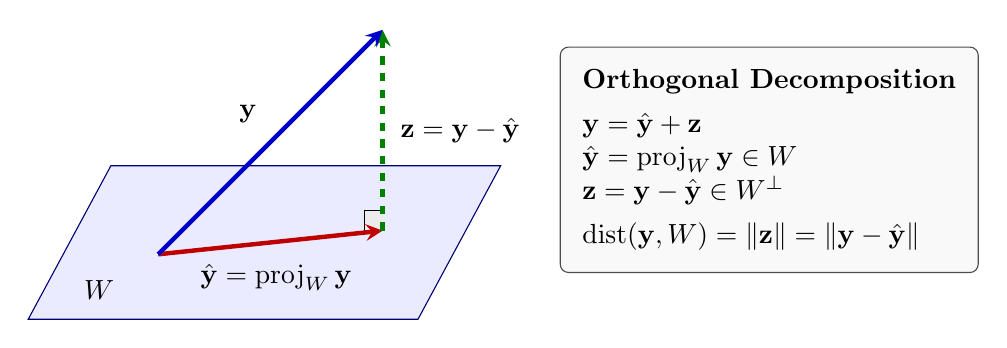
\begin{tikzpicture}[scale=1.5]
    % Layer 1: Fills
    \fill[blue!8] (-0.4,-0.4) -- (2.9,-0.4) -- (3.6,0.9) -- (0.3,0.9) -- cycle;
    \fill[gray!15] (2.45,0.35) -- (2.45,0.52) -- (2.6,0.52) -- (2.6,0.35) -- cycle;

    % Layer 2: Subspace borders and right-angle marker
    \draw[thin, blue!45!black] (-0.4,-0.4) -- (2.9,-0.4) -- (3.6,0.9) -- (0.3,0.9) -- cycle;
    \draw[thin, black] (2.45,0.35) -- (2.45,0.52) -- (2.6,0.52);

    % Layer 3: Primary vectors
    \draw[->, >=stealth, ultra thick, red!75!black] (0.7,0.15) -- (2.6,0.35);
    \draw[->, >=stealth, ultra thick, green!50!black, dashed] (2.6,0.35) -- (2.6,2.05);
    \draw[->, >=stealth, ultra thick, blue!80!black] (0.7,0.15) -- (2.6,2.05);

    % Layer 4: Labels and single-node multiline summary
    \node[black] at (0.2, -0.15) {$W$};
    \node[black, above left=2pt] at (1.65, 1.15) {$\mathbf{y}$};
    \node[black, below=3pt] at (1.7, 0.22) {$\hat{\mathbf{y}} = \operatorname{proj}_W \mathbf{y}$};
    \node[black, right=3pt] at (2.6, 1.2) {$\mathbf{z} = \mathbf{y} - \hat{\mathbf{y}}$};

    \node[anchor=west, draw=black!70, fill=gray!5, rounded corners=3pt, align=left, inner sep=8pt, text=black] at (4.1, 0.95) {
        \textbf{Orthogonal Decomposition} \\[4pt]
        $\mathbf{y} = \hat{\mathbf{y}} + \mathbf{z}$ \\
        $\hat{\mathbf{y}} = \operatorname{proj}_W \mathbf{y} \in W$ \\
        $\mathbf{z} = \mathbf{y} - \hat{\mathbf{y}} \in W^\perp$ \\[4pt]
        $\operatorname{dist}(\mathbf{y}, W) = \|\mathbf{z}\| = \|\mathbf{y} - \hat{\mathbf{y}}\|$
    };
\end{tikzpicture}
\end{center}

\begin{definition}[Orthogonal Projection and Decomposition]
Let $W$ be a subspace of $\R^n$ with an orthogonal basis $\{\mathbf{u}_1, \dots, \mathbf{u}_p\}$. Each $\mathbf{y} \in \R^n$ can be written uniquely as $\mathbf{y} = \hat{\mathbf{y}} + \mathbf{z}$, where $\hat{\mathbf{y}} \in W$ is the orthogonal projection of $\mathbf{y}$ onto $W$:
\[
\hat{\mathbf{y}} = \operatorname{proj}_W \mathbf{y} = \frac{\mathbf{y} \cdot \mathbf{u}_1}{\mathbf{u}_1 \cdot \mathbf{u}_1}\mathbf{u}_1 + \frac{\mathbf{y} \cdot \mathbf{u}_2}{\mathbf{u}_2 \cdot \mathbf{u}_2}\mathbf{u}_2 + \dots + \frac{\mathbf{y} \cdot \mathbf{u}_p}{\mathbf{u}_p \cdot \mathbf{u}_p}\mathbf{u}_p,
\]
and $\mathbf{z} = \mathbf{y} - \hat{\mathbf{y}}$ lies in $W^\perp$. By the Best Approximation Theorem, $\hat{\mathbf{y}}$ is the unique point in $W$ closest to $\mathbf{y}$, and $\operatorname{dist}(\mathbf{y}, W) = \|\mathbf{y} - \hat{\mathbf{y}}\| = \|\mathbf{z}\|$.
\end{definition}

\begin{definition}[Orthonormal Columns and Projection Matrix]
If $U = [\mathbf{u}_1 \ \cdots \ \mathbf{u}_p] \in \R^{n \times p}$ has orthonormal columns ($U^T U = I_p$), then the orthogonal projection onto $W = \operatorname{Col}(U)$ simplifies to:
\[
\operatorname{proj}_W \mathbf{y} = (\mathbf{y} \cdot \mathbf{u}_1)\mathbf{u}_1 + \dots + (\mathbf{y} \cdot \mathbf{u}_p)\mathbf{u}_p = UU^T \mathbf{y} = U(U^T \mathbf{y}).
\]
\end{definition}

\subsection{Problem Types and General Approach}

\begin{description}[style=nextline, leftmargin=1.5em, labelindent=0em]
    \item[Type 1: Verifying Orthogonality and Computing Projections (Problems 1--6)]
    \begin{itemize}
        \item \textbf{Concepts Covered:} Pairwise dot-product orthogonality checks ($\mathbf{u}_i \cdot \mathbf{u}_j = 0$ for $i \neq j$), the Orthogonal Projection Formula in $\R^3$ and $\R^4$, identifying membership ($\hat{\mathbf{y}} = \mathbf{y} \iff \mathbf{y} \in W$ and $\hat{\mathbf{y}} = \mathbf{0} \iff \mathbf{y} \in W^\perp$), and detecting the \emph{Non-Orthogonal Basis Trap}.
        \item \textbf{General Strategic Workflow:} Always begin by computing $\mathbf{u}_i \cdot \mathbf{u}_j$ for every distinct pair of basis vectors. Only if all pairwise dot products vanish may you apply $\sum \frac{\mathbf{y}\cdot\mathbf{u}_i}{\mathbf{u}_i\cdot\mathbf{u}_i}\mathbf{u}_i$. Simplify scalar fractions before multiplying into vectors, and check $(\mathbf{y} - \hat{\mathbf{y}}) \cdot \mathbf{u}_i = 0$ at the end.
    \end{itemize}

    \item[Type 2: Orthogonal Decomposition Theorem (Problems 7--11)]
    \begin{itemize}
        \item \textbf{Concepts Covered:} Expressing $\mathbf{y} = \hat{\mathbf{y}} + \mathbf{z}$ with $\hat{\mathbf{y}} \in W$ and $\mathbf{z} \in W^\perp$, uniqueness of decomposition, recovering $\mathbf{y}$ from partial projection data, and the \emph{Zero-Check Sanity Trick}.
        \item \textbf{General Strategic Workflow:} First verify basis orthogonality. Second, compute $\hat{\mathbf{y}} = \operatorname{proj}_W \mathbf{y}$. Third, subtract in the correct order $\mathbf{z} = \mathbf{y} - \hat{\mathbf{y}}$ (avoiding the $\hat{\mathbf{y}} - \mathbf{y}$ sign error). Finally, verify $\mathbf{z} \cdot \mathbf{u}_i = 0$ for all $i$.
    \end{itemize}

    \item[Type 3: Best Approximation Theorem and Closest Point (Problems 12--15)]
    \begin{itemize}
        \item \textbf{Concepts Covered:} Identifying $\hat{\mathbf{y}} = \operatorname{proj}_W \mathbf{y}$ as the unique closest point in $W$ to $\mathbf{y}$, minimizing $\|\mathbf{y} - \mathbf{v}\|$ over $\mathbf{v} \in W$, and verifying optimality via the Pythagorean relation $\|\mathbf{y} - \mathbf{v}\|^2 = \|\mathbf{y} - \hat{\mathbf{y}}\|^2 + \|\hat{\mathbf{y}} - \mathbf{v}\|^2$.
        \item \textbf{General Strategic Workflow:} Translate phrases like ``closest point'' or ``best approximation'' directly into $\hat{\mathbf{y}} = \operatorname{proj}_W \mathbf{y}$. Ensure the output is a \emph{vector} in $W$, not a scalar.
    \end{itemize}

    \item[Type 4: Distance from a Vector to a Subspace (Problems 16--19)]
    \begin{itemize}
        \item \textbf{Concepts Covered:} Computing $\operatorname{dist}(\mathbf{y}, W) = \|\mathbf{z}\| = \|\mathbf{y} - \hat{\mathbf{y}}\| = \sqrt{\mathbf{z} \cdot \mathbf{z}}$, distances to lines and planes in $\R^3$ and $\R^4$, and distinguishing distance (scalar) from closest point (vector).
        \item \textbf{General Strategic Workflow:} Compute $\hat{\mathbf{y}}$, form $\mathbf{z} = \mathbf{y} - \hat{\mathbf{y}}$, verify $\mathbf{z} \cdot \mathbf{u}_i = 0$, and take the Euclidean norm $\|\mathbf{z}\|$ (never $\|\hat{\mathbf{y}}\|$). Factor out common denominators before summing squares under the radical.
    \end{itemize}

    \item[Type 5: Orthonormal Bases and Projection Matrices (Problems 20--24)]
    \begin{itemize}
        \item \textbf{Concepts Covered:} Simplified orthonormal projection $\hat{\mathbf{y}} = \sum (\mathbf{y}\cdot\mathbf{u}_i)\mathbf{u}_i$, matrix properties $U^T U = I_p$ vs.\ $UU^T \neq I_n$ for rectangular $U$, associativity trick $U(U^T \mathbf{y})$, symmetry ($P^T = P$) and idempotence ($P^2 = P$) of $P = UU^T$, and the complementary projector $I_n - UU^T$ onto $W^\perp$.
        \item \textbf{General Strategic Workflow:} Verify unit length ($\|\mathbf{u}_i\| = 1$) and orthogonality ($\mathbf{u}_i \cdot \mathbf{u}_j = 0$). Use $U(U^T \mathbf{y})$ to compute projections rapidly without forming the $n \times n$ matrix $UU^T$ unless explicitly requested. Remember that $UU^T = I_n$ holds only when $U$ is square ($p = n$).
    \end{itemize}

    \item[Type 6: Conceptual True/False, Proofs, Diagnostic Flaws, and Modeling (Problems 25--30)]
    \begin{itemize}
        \item \textbf{Concepts Covered:} Rigorous True/False justifications on $W^\perp$ and projections, proving idempotence and fixed-point characterizations, diagnosing fatal flaws (non-orthogonal basis, $\|\hat{\mathbf{y}}\|$ distance error, $\hat{\mathbf{y}} - \mathbf{y}$ sign error, $UU^T = I$ assumption), and orthogonal regression residuals ($X^T \mathbf{z} = \mathbf{0}$).
        \item \textbf{General Strategic Workflow:} Test every claim against definitions and theorems. In flaw-finding problems, check basis orthogonality first, subtraction order second, norm target third, and matrix dimensions fourth.
    \end{itemize}
\end{description}

\renewcommand{\arraystretch}{1.5}
\begin{tabularx}{\textwidth}{>{\bfseries}l X c}
\toprule
Concept / Problem Type & Key Formula or Principle & Assigned Problems \\
\midrule
Verifying Orthogonality \& Projection & $\mathbf{u}_i \cdot \mathbf{u}_j = 0 \ (i \neq j)$; $\hat{\mathbf{y}} = \sum \frac{\mathbf{y}\cdot\mathbf{u}_i}{\mathbf{u}_i\cdot\mathbf{u}_i}\mathbf{u}_i$ & 1--6 \\
Orthogonal Decomposition & $\mathbf{y} = \hat{\mathbf{y}} + \mathbf{z}$, $\hat{\mathbf{y}} \in W$, $\mathbf{z} = \mathbf{y} - \hat{\mathbf{y}} \in W^\perp$ & 7--11 \\
Best Approximation Theorem & $\hat{\mathbf{y}} = \arg\min_{\mathbf{v} \in W} \|\mathbf{y} - \mathbf{v}\|$ & 12--15 \\
Distance to a Subspace & $\operatorname{dist}(\mathbf{y}, W) = \|\mathbf{y} - \hat{\mathbf{y}}\| = \|\mathbf{z}\|$ & 16--19 \\
Orthonormal Matrices ($U^T U$ vs.\ $UU^T$) & $U^T U = I_p$; $\operatorname{proj}_W \mathbf{y} = UU^T \mathbf{y} = U(U^T \mathbf{y})$ & 20--24 \\
Conceptual, Diagnostic \& Modeling & Proofs, T/F, ``Find the Flaw'', $X^T(\mathbf{y} - \hat{\mathbf{y}}) = \mathbf{0}$ & 25--30 \\
\bottomrule
\end{tabularx}

\newpage

\section{Problem Sets}

\subsection{Type 1: Verifying Orthogonality and Computing Projections (Problems 1--6)}

\textbf{Problem 1.} Verify that $\{\mathbf{u}_1, \mathbf{u}_2\}$ is an orthogonal set, and find the orthogonal projection of $\mathbf{y}$ onto $W = \operatorname{Span}\{\mathbf{u}_1, \mathbf{u}_2\}$, where
\[
\mathbf{y} = \begin{bmatrix} 2 \\ -3 \\ 5 \end{bmatrix}, \quad \mathbf{u}_1 = \begin{bmatrix} 1 \\ 1 \\ 0 \end{bmatrix}, \quad \mathbf{u}_2 = \begin{bmatrix} -1 \\ 1 \\ 0 \end{bmatrix}.
\]

\textbf{Problem 2.} Verify that $\{\mathbf{u}_1, \mathbf{u}_2\}$ is an orthogonal set, and compute $\operatorname{proj}_W \mathbf{y}$ for $W = \operatorname{Span}\{\mathbf{u}_1, \mathbf{u}_2\}$, where
\[
\mathbf{y} = \begin{bmatrix} 3 \\ 1 \\ -2 \end{bmatrix}, \quad \mathbf{u}_1 = \begin{bmatrix} 2 \\ -1 \\ 1 \end{bmatrix}, \quad \mathbf{u}_2 = \begin{bmatrix} 1 \\ 1 \\ -1 \end{bmatrix}.
\]

\textbf{Problem 3.} Verify that $\{\mathbf{u}_1, \mathbf{u}_2\}$ is an orthogonal set, compute $\operatorname{proj}_W \mathbf{y}$ onto $W = \operatorname{Span}\{\mathbf{u}_1, \mathbf{u}_2\}$, and state what your result implies geometrically about $\mathbf{y}$ relative to $W$:
\[
\mathbf{y} = \begin{bmatrix} -1 \\ 5 \\ -3 \end{bmatrix}, \quad \mathbf{u}_1 = \begin{bmatrix} 1 \\ 2 \\ -1 \end{bmatrix}, \quad \mathbf{u}_2 = \begin{bmatrix} 3 \\ -1 \\ 1 \end{bmatrix}.
\]

\textbf{Problem 4.} Verify that $\{\mathbf{u}_1, \mathbf{u}_2, \mathbf{u}_3\}$ is an orthogonal set in $\R^4$, and find $\operatorname{proj}_W \mathbf{y}$ where $W = \operatorname{Span}\{\mathbf{u}_1, \mathbf{u}_2, \mathbf{u}_3\}$:
\[
\mathbf{y} = \begin{bmatrix} 2 \\ 0 \\ -4 \\ 6 \end{bmatrix}, \quad \mathbf{u}_1 = \begin{bmatrix} 1 \\ 1 \\ 1 \\ 1 \end{bmatrix}, \quad \mathbf{u}_2 = \begin{bmatrix} 1 \\ -1 \\ 1 \\ -1 \end{bmatrix}, \quad \mathbf{u}_3 = \begin{bmatrix} 1 \\ 1 \\ -1 \\ -1 \end{bmatrix}.
\]

\textbf{Problem 5.} Verify that $\{\mathbf{u}_1, \mathbf{u}_2\}$ is an orthogonal set, compute $\operatorname{proj}_W \mathbf{y}$ onto $W = \operatorname{Span}\{\mathbf{u}_1, \mathbf{u}_2\}$, and interpret the result geometrically:
\[
\mathbf{y} = \begin{bmatrix} 2 \\ 0 \\ -2 \end{bmatrix}, \quad \mathbf{u}_1 = \begin{bmatrix} 1 \\ 1 \\ 1 \end{bmatrix}, \quad \mathbf{u}_2 = \begin{bmatrix} 1 \\ -2 \\ 1 \end{bmatrix}.
\]

\textbf{Problem 6.} Consider the vectors
\[
\mathbf{y} = \begin{bmatrix} 4 \\ 1 \\ 2 \end{bmatrix}, \quad \mathbf{u}_1 = \begin{bmatrix} 1 \\ 2 \\ 0 \end{bmatrix}, \quad \mathbf{u}_2 = \begin{bmatrix} 1 \\ 0 \\ 1 \end{bmatrix},
\]
and let $W = \operatorname{Span}\{\mathbf{u}_1, \mathbf{u}_2\}$. Determine whether the formula $\tilde{\mathbf{y}} = \frac{\mathbf{y}\cdot\mathbf{u}_1}{\mathbf{u}_1\cdot\mathbf{u}_1}\mathbf{u}_1 + \frac{\mathbf{y}\cdot\mathbf{u}_2}{\mathbf{u}_2\cdot\mathbf{u}_2}\mathbf{u}_2$ produces the true orthogonal projection $\operatorname{proj}_W \mathbf{y}$. Justify your conclusion both by checking the basis vectors and by testing whether $\mathbf{y} - \tilde{\mathbf{y}}$ is orthogonal to $W$.

\subsection{Type 2: Orthogonal Decomposition Theorem (Problems 7--11)}

\textbf{Problem 7.} Decompose $\mathbf{y} = \begin{bmatrix} 5 \\ 3 \end{bmatrix}$ as $\mathbf{y} = \hat{\mathbf{y}} + \mathbf{z}$, where $\hat{\mathbf{y}} \in W$ and $\mathbf{z} \in W^\perp$, for $W = \operatorname{Span}\left\{\begin{bmatrix} 2 \\ 1 \end{bmatrix}\right\}$. Verify your answer using the zero-check $\mathbf{z} \cdot \mathbf{u} = 0$.

\textbf{Problem 8.} Let $W$ be the subspace spanned by $\mathbf{u}_1$ and $\mathbf{u}_2$. Write $\mathbf{y}$ as the sum of a vector $\hat{\mathbf{y}}$ in $W$ and a vector $\mathbf{z}$ orthogonal to $W$:
\[
\mathbf{y} = \begin{bmatrix} 1 \\ 3 \\ 5 \end{bmatrix}, \quad \mathbf{u}_1 = \begin{bmatrix} 2 \\ 1 \\ 1 \end{bmatrix}, \quad \mathbf{u}_2 = \begin{bmatrix} -1 \\ 1 \\ 1 \end{bmatrix}.
\]

\textbf{Problem 9.} Let $W = \operatorname{Span}\{\mathbf{u}_1, \mathbf{u}_2\}$. Find the orthogonal decomposition $\mathbf{y} = \hat{\mathbf{y}} + \mathbf{z}$ with $\hat{\mathbf{y}} \in W$ and $\mathbf{z} \in W^\perp$, and verify $\mathbf{z} \cdot \mathbf{u}_1 = \mathbf{z} \cdot \mathbf{u}_2 = 0$:
\[
\mathbf{y} = \begin{bmatrix} 4 \\ -1 \\ 2 \end{bmatrix}, \quad \mathbf{u}_1 = \begin{bmatrix} 1 \\ 2 \\ -2 \end{bmatrix}, \quad \mathbf{u}_2 = \begin{bmatrix} 2 \\ 1 \\ 2 \end{bmatrix}.
\]

\textbf{Problem 10.} Let $W = \operatorname{Span}\{\mathbf{u}_1, \mathbf{u}_2\} \subseteq \R^4$. Write $\mathbf{y}$ as $\hat{\mathbf{y}} + \mathbf{z}$ with $\hat{\mathbf{y}} \in W$ and $\mathbf{z} \in W^\perp$:
\[
\mathbf{y} = \begin{bmatrix} 1 \\ 2 \\ -1 \\ 4 \end{bmatrix}, \quad \mathbf{u}_1 = \begin{bmatrix} 1 \\ 0 \\ 1 \\ 0 \end{bmatrix}, \quad \mathbf{u}_2 = \begin{bmatrix} 1 \\ 2 \\ -1 \\ 0 \end{bmatrix}.
\]

\textbf{Problem 11.} Suppose $\mathbf{y} \in \R^4$ has orthogonal decomposition $\mathbf{y} = \hat{\mathbf{y}} + \mathbf{z}$ with respect to $W = \operatorname{Span}\{\mathbf{u}_1, \mathbf{u}_2\}$, where
\[
\mathbf{u}_1 = \begin{bmatrix} 2 \\ 1 \\ 0 \\ -1 \end{bmatrix}, \quad \mathbf{u}_2 = \begin{bmatrix} 1 \\ -1 \\ 2 \\ 1 \end{bmatrix}, \quad \mathbf{z} = \begin{bmatrix} 2 \\ 0 \\ -3 \\ 4 \end{bmatrix}.
\]
It is also known that $\mathbf{y} \cdot \mathbf{u}_1 = 12$ and $\mathbf{y} \cdot \mathbf{u}_2 = -7$. Verify that $\{\mathbf{u}_1, \mathbf{u}_2\}$ is orthogonal and $\mathbf{z} \in W^\perp$, and then determine $\hat{\mathbf{y}}$ and $\mathbf{y}$.

\subsection{Type 3: Best Approximation Theorem and Closest Point (Problems 12--15)}

\textbf{Problem 12.} Find the closest point to $\mathbf{y}$ in the subspace $W = \operatorname{Span}\{\mathbf{v}_1, \mathbf{v}_2\} \subseteq \R^4$, where
\[
\mathbf{y} = \begin{bmatrix} 4 \\ 2 \\ 0 \\ 4 \end{bmatrix}, \quad \mathbf{v}_1 = \begin{bmatrix} 1 \\ 1 \\ 1 \\ -1 \end{bmatrix}, \quad \mathbf{v}_2 = \begin{bmatrix} 1 \\ -1 \\ 1 \\ 1 \end{bmatrix}.
\]

\textbf{Problem 13.} Let $\mathbf{y} = \begin{bmatrix} 2 \\ 7 \\ 1 \end{bmatrix}$, $\mathbf{v}_1 = \begin{bmatrix} 1 \\ 2 \\ 2 \end{bmatrix}$, $\mathbf{v}_2 = \begin{bmatrix} 2 \\ -2 \\ 1 \end{bmatrix}$, and $W = \operatorname{Span}\{\mathbf{v}_1, \mathbf{v}_2\}$.
\begin{enumerate}[label=(\alph*)]
    \item Find the best approximation $\hat{\mathbf{y}}$ to $\mathbf{y}$ in $W$.
    \item Let $\mathbf{v} = \mathbf{v}_1 + \mathbf{v}_2 \in W$. Compute $\|\mathbf{y} - \hat{\mathbf{y}}\|$ and $\|\mathbf{y} - \mathbf{v}\|$, and verify the Pythagorean identity $\|\mathbf{y} - \mathbf{v}\|^2 = \|\mathbf{y} - \hat{\mathbf{y}}\|^2 + \|\hat{\mathbf{y}} - \mathbf{v}\|^2$.
\end{enumerate}

\textbf{Problem 14.} Find the scalar $c \in \R$ and the vector $\hat{\mathbf{y}} = c\mathbf{v}$ that minimize $\|\mathbf{y} - c\mathbf{v}\|$ for
\[
\mathbf{y} = \begin{bmatrix} -2 \\ 5 \\ 4 \end{bmatrix}, \quad \mathbf{v} = \begin{bmatrix} 1 \\ -2 \\ 2 \end{bmatrix}.
\]

\textbf{Problem 15.} Find the closest point to $\mathbf{y}$ in the subspace $W = \operatorname{Span}\{\mathbf{v}_1, \mathbf{v}_2, \mathbf{v}_3\} \subseteq \R^4$, where
\[
\mathbf{y} = \begin{bmatrix} 5 \\ -1 \\ 3 \\ 1 \end{bmatrix}, \quad \mathbf{v}_1 = \begin{bmatrix} 1 \\ 1 \\ 0 \\ 0 \end{bmatrix}, \quad \mathbf{v}_2 = \begin{bmatrix} 1 \\ -1 \\ 1 \\ 1 \end{bmatrix}, \quad \mathbf{v}_3 = \begin{bmatrix} 0 \\ 0 \\ 1 \\ -1 \end{bmatrix}.
\]

\subsection{Type 4: Distance from a Vector to a Subspace (Problems 16--19)}

\textbf{Problem 16.} Find the distance from $\mathbf{y}$ to the plane in $\R^3$ spanned by $\mathbf{u}_1$ and $\mathbf{u}_2$:
\[
\mathbf{y} = \begin{bmatrix} 3 \\ 4 \\ 1 \end{bmatrix}, \quad \mathbf{u}_1 = \begin{bmatrix} 1 \\ -2 \\ 2 \end{bmatrix}, \quad \mathbf{u}_2 = \begin{bmatrix} 2 \\ 1 \\ 0 \end{bmatrix}.
\]

\textbf{Problem 17.} Find the distance from $\mathbf{y}$ to the subspace $W = \operatorname{Span}\{\mathbf{u}_1, \mathbf{u}_2\} \subseteq \R^3$:
\[
\mathbf{y} = \begin{bmatrix} 4 \\ -2 \\ 9 \end{bmatrix}, \quad \mathbf{u}_1 = \begin{bmatrix} 1 \\ -3 \\ 2 \end{bmatrix}, \quad \mathbf{u}_2 = \begin{bmatrix} 3 \\ 1 \\ 0 \end{bmatrix}.
\]

\textbf{Problem 18.} Find the distance from $\mathbf{y} = \begin{bmatrix} 3 \\ -1 \\ 4 \\ 2 \end{bmatrix}$ to the line $L = \operatorname{Span}\left\{\begin{bmatrix} 1 \\ 1 \\ 1 \\ 1 \end{bmatrix}\right\}$ in $\R^4$.

\textbf{Problem 19.} Let $\mathbf{y} = \begin{bmatrix} 1 \\ 3 \\ -2 \\ 4 \end{bmatrix}$, $\mathbf{u}_1 = \begin{bmatrix} 1 \\ 0 \\ 1 \\ 0 \end{bmatrix}$, $\mathbf{u}_2 = \begin{bmatrix} 0 \\ 1 \\ 0 \\ -1 \end{bmatrix}$, and $W = \operatorname{Span}\{\mathbf{u}_1, \mathbf{u}_2\}$.
\begin{enumerate}[label=(\alph*)]
    \item Find the closest point in $W$ to $\mathbf{y}$.
    \item Find the distance from $\mathbf{y}$ to $W$, and briefly explain why parts (a) and (b) produce different types of mathematical objects.
\end{enumerate}

\subsection{Type 5: Orthonormal Bases and Projection Matrices (Problems 20--24)}

\textbf{Problem 20.} Let $\mathbf{y} = \begin{bmatrix} 6 \\ 3 \\ -3 \end{bmatrix}$, $\mathbf{u}_1 = \begin{bmatrix} 2/3 \\ -2/3 \\ 1/3 \end{bmatrix}$, $\mathbf{u}_2 = \begin{bmatrix} 1/3 \\ 2/3 \\ 2/3 \end{bmatrix}$, $W = \operatorname{Span}\{\mathbf{u}_1, \mathbf{u}_2\}$, and $U = [\mathbf{u}_1 \ \mathbf{u}_2]$.
\begin{enumerate}[label=(\alph*)]
    \item Verify that $\{\mathbf{u}_1, \mathbf{u}_2\}$ is orthonormal, and compute $U^T U$ and $UU^T$.
    \item Compute $\operatorname{proj}_W \mathbf{y}$ using the simplified orthonormal projection formula, and verify that it matches $(UU^T)\mathbf{y}$.
\end{enumerate}

\textbf{Problem 21.} Let
\[
U = \frac{1}{2}\begin{bmatrix} 1 & 1 \\ 1 & -1 \\ 1 & 1 \\ 1 & -1 \end{bmatrix} \quad \text{and} \quad \mathbf{y} = \begin{bmatrix} 4 \\ 0 \\ 2 \\ -2 \end{bmatrix}.
\]
\begin{enumerate}[label=(\alph*)]
    \item Verify that $U$ has orthonormal columns by computing $U^T U$.
    \item Compute $\operatorname{proj}_{\operatorname{Col}(U)} \mathbf{y}$ via the associative form $U(U^T \mathbf{y})$ without constructing the $4 \times 4$ matrix $UU^T$.
    \item Explicitly compute $UU^T$ and confirm that $(UU^T)\mathbf{y}$ yields the same vector as part (b).
\end{enumerate}

\textbf{Problem 22.} Let
\[
U = \begin{bmatrix} 1/\sqrt{2} & 1/\sqrt{6} \\ -1/\sqrt{2} & 1/\sqrt{6} \\ 0 & -2/\sqrt{6} \end{bmatrix} \quad \text{and} \quad \mathbf{y} = \begin{bmatrix} 3 \\ 1 \\ 2 \end{bmatrix}.
\]
\begin{enumerate}[label=(\alph*)]
    \item Show that $U^T U = I_2$.
    \item Compute the projection matrix $P = UU^T$ onto $W = \operatorname{Col}(U)$, and verify directly that $P^T = P$ and $P^2 = P$.
    \item Compute $\operatorname{proj}_W \mathbf{y} = P\mathbf{y}$ and find $\operatorname{dist}(\mathbf{y}, W)$.
\end{enumerate}

\textbf{Problem 23.} Consider the matrices
\[
U = \begin{bmatrix} 3/5 & -4/5 \\ 4/5 & 3/5 \end{bmatrix} \quad \text{and} \quad V = \begin{bmatrix} 3/5 \\ 4/5 \end{bmatrix}.
\]
\begin{enumerate}[label=(\alph*)]
    \item Compute $U^T U$ and $UU^T$, and determine $\operatorname{proj}_{\operatorname{Col}(U)} \mathbf{y}$ for any $\mathbf{y} \in \R^2$.
    \item Compute $V^T V$ and $VV^T$, and find $\operatorname{proj}_{\operatorname{Col}(V)} \mathbf{y}$ for $\mathbf{y} = \begin{bmatrix} 5 \\ 0 \end{bmatrix}$.
    \item Explain why $UU^T = I_2$ holds for $U$, whereas $VV^T \neq I_2$ for $V$.
\end{enumerate}

\textbf{Problem 24.} Let
\[
U = \frac{1}{2}\begin{bmatrix} 1 & 1 & 1 \\ 1 & -1 & -1 \\ 1 & 1 & -1 \\ 1 & -1 & 1 \end{bmatrix} \quad \text{and} \quad \mathbf{y} = \begin{bmatrix} 5 \\ 3 \\ 3 \\ -3 \end{bmatrix},
\]
and let $W = \operatorname{Col}(U)$.
\begin{enumerate}[label=(\alph*)]
    \item Verify that $U^T U = I_3$.
    \item Compute $\hat{\mathbf{y}} = U(U^T \mathbf{y})$ and $\mathbf{z} = (I_4 - UU^T)\mathbf{y}$.
    \item Verify that $U^T \mathbf{z} = \mathbf{0}$, and explain why $I_4 - UU^T$ is the projection matrix onto $W^\perp$.
\end{enumerate}

\subsection{Type 6: Conceptual, Diagnostic, and Modeling Problems (Problems 25--30)}

\textbf{Problem 25.} Determine whether each statement is True or False. Justify each answer rigorously using definitions or theorems from Section 6.3.
\begin{enumerate}[label=(\alph*)]
    \item If $\mathbf{z}$ is orthogonal to both $\mathbf{u}_1$ and $\mathbf{u}_2$, and $W = \operatorname{Span}\{\mathbf{u}_1, \mathbf{u}_2\}$, then $\mathbf{z}$ must be in $W^\perp$.
    \item For every $\mathbf{y} \in \R^n$ and every subspace $W \subseteq \R^n$, the vector $\mathbf{y} - \operatorname{proj}_W \mathbf{y}$ is orthogonal to $W$.
    \item If $\mathbf{y} \in W$, then $\operatorname{proj}_W \mathbf{y} = \mathbf{0}$.
    \item If $U$ is an $n \times p$ matrix with orthonormal columns and $p < n$, then $UU^T = I_n$.
\end{enumerate}

\textbf{Problem 26.} Let $W$ be a subspace of $\R^n$. Using the Orthogonal Decomposition Theorem, prove the following properties:
\begin{enumerate}[label=(\alph*)]
    \item $\operatorname{proj}_W(\operatorname{proj}_W \mathbf{y}) = \operatorname{proj}_W \mathbf{y}$ for every $\mathbf{y} \in \R^n$.
    \item $\operatorname{proj}_W \mathbf{y} = \mathbf{y}$ if and only if $\mathbf{y} \in W$.
    \item $\|\mathbf{y}\|^2 = \|\operatorname{proj}_W \mathbf{y}\|^2 + \|\mathbf{y} - \operatorname{proj}_W \mathbf{y}\|^2$ for every $\mathbf{y} \in \R^n$.
\end{enumerate}

\textbf{Problem 27 (Diagnostic: Find the Flaw).} A student is asked to find $\operatorname{proj}_W \mathbf{y}$ for $\mathbf{y} = \begin{bmatrix} 3 \\ 1 \\ 2 \end{bmatrix}$ onto $W = \operatorname{Span}\{\mathbf{u}_1, \mathbf{u}_2\}$, where $\mathbf{u}_1 = \begin{bmatrix} 1 \\ 0 \\ 1 \end{bmatrix}$ and $\mathbf{u}_2 = \begin{bmatrix} 0 \\ 1 \\ 1 \end{bmatrix}$. The student writes:
\[
\hat{\mathbf{y}} = \frac{\mathbf{y}\cdot\mathbf{u}_1}{\mathbf{u}_1\cdot\mathbf{u}_1}\mathbf{u}_1 + \frac{\mathbf{y}\cdot\mathbf{u}_2}{\mathbf{u}_2\cdot\mathbf{u}_2}\mathbf{u}_2 = \frac{5}{2}\begin{bmatrix} 1 \\ 0 \\ 1 \end{bmatrix} + \frac{3}{2}\begin{bmatrix} 0 \\ 1 \\ 1 \end{bmatrix} = \begin{bmatrix} 5/2 \\ 3/2 \\ 4 \end{bmatrix}.
\]
\begin{enumerate}[label=(\alph*)]
    \item Identify the critical flaw in the student's work.
    \item Verify algebraically that $\begin{bmatrix} 5/2 \\ 3/2 \\ 4 \end{bmatrix}$ is not the true orthogonal projection.
    \item Find the true projection $\hat{\mathbf{y}} = c_1 \mathbf{u}_1 + c_2 \mathbf{u}_2$ directly from the orthogonality conditions $(\mathbf{y} - \hat{\mathbf{y}}) \cdot \mathbf{u}_1 = 0$ and $(\mathbf{y} - \hat{\mathbf{y}}) \cdot \mathbf{u}_2 = 0$.
\end{enumerate}

\textbf{Problem 28 (Diagnostic: Find the Flaw).} A student attempts to find the orthogonal decomposition of $\mathbf{y} = \begin{bmatrix} 2 \\ 6 \end{bmatrix}$ with respect to $W = \operatorname{Span}\left\{\begin{bmatrix} 3 \\ 1 \end{bmatrix}\right\}$ and the distance from $\mathbf{y}$ to $W$. The student writes:
\[
\hat{\mathbf{y}} = \frac{12}{10}\begin{bmatrix} 3 \\ 1 \end{bmatrix} = \begin{bmatrix} 18/5 \\ 6/5 \end{bmatrix}, \qquad \mathbf{z} = \hat{\mathbf{y}} - \mathbf{y} = \begin{bmatrix} 8/5 \\ -24/5 \end{bmatrix}, \qquad \operatorname{dist}(\mathbf{y}, W) = \|\hat{\mathbf{y}}\| = \frac{6\sqrt{10}}{5}.
\]
\begin{enumerate}[label=(\alph*)]
    \item Identify both errors in the student's solution.
    \item Provide the corrected orthogonal decomposition $\mathbf{y} = \hat{\mathbf{y}} + \mathbf{z}$ and the true distance $\operatorname{dist}(\mathbf{y}, W)$.
\end{enumerate}

\textbf{Problem 29 (Diagnostic: Find the Flaw).} Let $U = \begin{bmatrix} 1/\sqrt{5} & 0 \\ 2/\sqrt{5} & 0 \\ 0 & 1 \end{bmatrix}$ and $\mathbf{y} = \begin{bmatrix} 5 \\ 0 \\ 3 \end{bmatrix}$. A student writes: ``Because the columns of $U$ are orthonormal, $U$ is an orthogonal matrix and $UU^T = I_3$. Thus $\operatorname{proj}_{\operatorname{Col}(U)} \mathbf{y} = UU^T\mathbf{y} = \mathbf{y} = \begin{bmatrix} 5 \\ 0 \\ 3 \end{bmatrix}$.''
\begin{enumerate}[label=(\alph*)]
    \item Identify the fatal conceptual flaw in the student's argument.
    \item Compute $U^T U$, $UU^T$, and the true projection $\operatorname{proj}_{\operatorname{Col}(U)} \mathbf{y}$.
    \item Find a non-zero vector $\mathbf{w} \in \R^3$ such that $UU^T\mathbf{w} = \mathbf{0}$.
\end{enumerate}

\textbf{Problem 30 (Linear Modeling Application).} In a linear model $\mathbf{y} \approx \beta_1 \mathbf{x}_1 + \beta_2 \mathbf{x}_2$, suppose the target vector is $\mathbf{y} = \begin{bmatrix} 5 \\ 3 \\ 5 \\ -1 \end{bmatrix}$ and the feature columns of the design matrix $X = [\mathbf{x}_1 \ \mathbf{x}_2]$ are
\[
\mathbf{x}_1 = \begin{bmatrix} 1 \\ 1 \\ -1 \\ -1 \end{bmatrix}, \quad \mathbf{x}_2 = \begin{bmatrix} 1 \\ -1 \\ 1 \\ -1 \end{bmatrix}.
\]
Let $W = \operatorname{Col}(X)$.
\begin{enumerate}[label=(\alph*)]
    \item Verify that $\mathbf{x}_1$ and $\mathbf{x}_2$ are orthogonal, and use the orthogonal projection formula to determine the optimal prediction $\hat{\mathbf{y}} = \operatorname{proj}_W \mathbf{y}$ and the optimal coefficient vector $\boldsymbol{\beta} = \begin{bmatrix} \beta_1 \\ \beta_2 \end{bmatrix}$.
    \item Find the residual vector $\mathbf{z} = \mathbf{y} - \hat{\mathbf{y}}$ and the minimum squared error $\|\mathbf{y} - \hat{\mathbf{y}}\|^2$.
    \item Verify directly that $X^T \mathbf{z} = \mathbf{0}$, confirming that the residual vector lies in the left null space of $X$.
\end{enumerate}

\newpage

\section{Detailed Solutions}

\subsection{Solutions to Type 1 Problems (Problems 1--6)}

\textbf{Problem 1 (Restated).} Verify that $\{\mathbf{u}_1, \mathbf{u}_2\}$ is an orthogonal set, and find the orthogonal projection of $\mathbf{y}$ onto $W = \operatorname{Span}\{\mathbf{u}_1, \mathbf{u}_2\}$, where
\[
\mathbf{y} = \begin{bmatrix} 2 \\ -3 \\ 5 \end{bmatrix}, \quad \mathbf{u}_1 = \begin{bmatrix} 1 \\ 1 \\ 0 \end{bmatrix}, \quad \mathbf{u}_2 = \begin{bmatrix} -1 \\ 1 \\ 0 \end{bmatrix}.
\]
\textbf{Solution.}
\textbf{Step 1: Verify orthogonality.}
\[
\mathbf{u}_1 \cdot \mathbf{u}_2 = (1)(-1) + (1)(1) + (0)(0) = -1 + 1 + 0 = 0.
\]
Since $\mathbf{u}_1 \cdot \mathbf{u}_2 = 0$, the set $\{\mathbf{u}_1, \mathbf{u}_2\}$ is orthogonal.

\textbf{Step 2: Compute dot products and project.}
\begin{align*}
\mathbf{y} \cdot \mathbf{u}_1 &= (2)(1) + (-3)(1) + (5)(0) = -1, & \mathbf{u}_1 \cdot \mathbf{u}_1 &= 1^2 + 1^2 + 0^2 = 2, \\
\mathbf{y} \cdot \mathbf{u}_2 &= (2)(-1) + (-3)(1) + (5)(0) = -5, & \mathbf{u}_2 \cdot \mathbf{u}_2 &= (-1)^2 + 1^2 + 0^2 = 2.
\end{align*}
Applying the orthogonal projection formula:
\[
\hat{\mathbf{y}} = \frac{\mathbf{y}\cdot\mathbf{u}_1}{\mathbf{u}_1\cdot\mathbf{u}_1}\mathbf{u}_1 + \frac{\mathbf{y}\cdot\mathbf{u}_2}{\mathbf{u}_2\cdot\mathbf{u}_2}\mathbf{u}_2 = -\frac{1}{2}\begin{bmatrix} 1 \\ 1 \\ 0 \end{bmatrix} - \frac{5}{2}\begin{bmatrix} -1 \\ 1 \\ 0 \end{bmatrix} = \begin{bmatrix} -1/2 + 5/2 \\ -1/2 - 5/2 \\ 0 \end{bmatrix} = \begin{bmatrix} 2 \\ -3 \\ 0 \end{bmatrix}.
\]
\textbf{Final Answer:} $\operatorname{proj}_W \mathbf{y} = \begin{bmatrix} 2 \\ -3 \\ 0 \end{bmatrix}$.

\medskip
\textbf{Problem 2 (Restated).} Verify that $\{\mathbf{u}_1, \mathbf{u}_2\}$ is an orthogonal set, and compute $\operatorname{proj}_W \mathbf{y}$ for $W = \operatorname{Span}\{\mathbf{u}_1, \mathbf{u}_2\}$, where
\[
\mathbf{y} = \begin{bmatrix} 3 \\ 1 \\ -2 \end{bmatrix}, \quad \mathbf{u}_1 = \begin{bmatrix} 2 \\ -1 \\ 1 \end{bmatrix}, \quad \mathbf{u}_2 = \begin{bmatrix} 1 \\ 1 \\ -1 \end{bmatrix}.
\]
\textbf{Solution.}
\textbf{Step 1: Verify orthogonality.}
\[
\mathbf{u}_1 \cdot \mathbf{u}_2 = (2)(1) + (-1)(1) + (1)(-1) = 2 - 1 - 1 = 0.
\]
Thus $\{\mathbf{u}_1, \mathbf{u}_2\}$ is orthogonal.

\textbf{Step 2: Compute dot products and project.}
\begin{align*}
\mathbf{y} \cdot \mathbf{u}_1 &= (3)(2) + (1)(-1) + (-2)(1) = 3, & \mathbf{u}_1 \cdot \mathbf{u}_1 &= 2^2 + (-1)^2 + 1^2 = 6, \\
\mathbf{y} \cdot \mathbf{u}_2 &= (3)(1) + (1)(1) + (-2)(-1) = 6, & \mathbf{u}_2 \cdot \mathbf{u}_2 &= 1^2 + 1^2 + (-1)^2 = 3.
\end{align*}
Substituting into the projection formula:
\[
\hat{\mathbf{y}} = \frac{3}{6}\begin{bmatrix} 2 \\ -1 \\ 1 \end{bmatrix} + \frac{6}{3}\begin{bmatrix} 1 \\ 1 \\ -1 \end{bmatrix} = \frac{1}{2}\begin{bmatrix} 2 \\ -1 \\ 1 \end{bmatrix} + 2\begin{bmatrix} 1 \\ 1 \\ -1 \end{bmatrix} = \begin{bmatrix} 1 + 2 \\ -1/2 + 2 \\ 1/2 - 2 \end{bmatrix} = \begin{bmatrix} 3 \\ 3/2 \\ -3/2 \end{bmatrix}.
\]
\textbf{Final Answer:} $\operatorname{proj}_W \mathbf{y} = \begin{bmatrix} 3 \\ 3/2 \\ -3/2 \end{bmatrix}$.

\medskip
\textbf{Problem 3 (Restated).} Verify that $\{\mathbf{u}_1, \mathbf{u}_2\}$ is an orthogonal set, compute $\operatorname{proj}_W \mathbf{y}$ onto $W = \operatorname{Span}\{\mathbf{u}_1, \mathbf{u}_2\}$, and state what your result implies geometrically about $\mathbf{y}$ relative to $W$:
\[
\mathbf{y} = \begin{bmatrix} -1 \\ 5 \\ -3 \end{bmatrix}, \quad \mathbf{u}_1 = \begin{bmatrix} 1 \\ 2 \\ -1 \end{bmatrix}, \quad \mathbf{u}_2 = \begin{bmatrix} 3 \\ -1 \\ 1 \end{bmatrix}.
\]
\textbf{Solution.}
\textbf{Step 1: Verify orthogonality.}
\[
\mathbf{u}_1 \cdot \mathbf{u}_2 = (1)(3) + (2)(-1) + (-1)(1) = 3 - 2 - 1 = 0.
\]
The set $\{\mathbf{u}_1, \mathbf{u}_2\}$ is orthogonal.

\textbf{Step 2: Compute dot products and project.}
\begin{align*}
\mathbf{y} \cdot \mathbf{u}_1 &= (-1)(1) + (5)(2) + (-3)(-1) = 12, & \mathbf{u}_1 \cdot \mathbf{u}_1 &= 1 + 4 + 1 = 6, \\
\mathbf{y} \cdot \mathbf{u}_2 &= (-1)(3) + (5)(-1) + (-3)(1) = -11, & \mathbf{u}_2 \cdot \mathbf{u}_2 &= 9 + 1 + 1 = 11.
\end{align*}
\[
\hat{\mathbf{y}} = \frac{12}{6}\begin{bmatrix} 1 \\ 2 \\ -1 \end{bmatrix} + \frac{-11}{11}\begin{bmatrix} 3 \\ -1 \\ 1 \end{bmatrix} = 2\begin{bmatrix} 1 \\ 2 \\ -1 \end{bmatrix} - \begin{bmatrix} 3 \\ -1 \\ 1 \end{bmatrix} = \begin{bmatrix} -1 \\ 5 \\ -3 \end{bmatrix}.
\]
\textbf{Final Answer:} $\operatorname{proj}_W \mathbf{y} = \begin{bmatrix} -1 \\ 5 \\ -3 \end{bmatrix} = \mathbf{y}$. Because $\hat{\mathbf{y}} = \mathbf{y}$, the vector $\mathbf{y}$ already lies in the subspace $W$.

\medskip
\textbf{Problem 4 (Restated).} Verify that $\{\mathbf{u}_1, \mathbf{u}_2, \mathbf{u}_3\}$ is an orthogonal set in $\R^4$, and find $\operatorname{proj}_W \mathbf{y}$ where $W = \operatorname{Span}\{\mathbf{u}_1, \mathbf{u}_2, \mathbf{u}_3\}$:
\[
\mathbf{y} = \begin{bmatrix} 2 \\ 0 \\ -4 \\ 6 \end{bmatrix}, \quad \mathbf{u}_1 = \begin{bmatrix} 1 \\ 1 \\ 1 \\ 1 \end{bmatrix}, \quad \mathbf{u}_2 = \begin{bmatrix} 1 \\ -1 \\ 1 \\ -1 \end{bmatrix}, \quad \mathbf{u}_3 = \begin{bmatrix} 1 \\ 1 \\ -1 \\ -1 \end{bmatrix}.
\]
\textbf{Solution.}
\textbf{Step 1: Verify pairwise orthogonality.}
\begin{align*}
\mathbf{u}_1 \cdot \mathbf{u}_2 &= 1 - 1 + 1 - 1 = 0, \\
\mathbf{u}_1 \cdot \mathbf{u}_3 &= 1 + 1 - 1 - 1 = 0, \\
\mathbf{u}_2 \cdot \mathbf{u}_3 &= 1 - 1 - 1 + 1 = 0.
\end{align*}
All three pairs are orthogonal.

\textbf{Step 2: Compute dot products and project.}
Each basis vector has squared norm $\mathbf{u}_i \cdot \mathbf{u}_i = 1^2 + 1^2 + 1^2 + 1^2 = 4$. Moreover:
\begin{align*}
\mathbf{y} \cdot \mathbf{u}_1 &= 2 + 0 - 4 + 6 = 4, \\
\mathbf{y} \cdot \mathbf{u}_2 &= 2 - 0 - 4 - 6 = -8, \\
\mathbf{y} \cdot \mathbf{u}_3 &= 2 + 0 + 4 - 6 = 0.
\end{align*}
Therefore:
\[
\hat{\mathbf{y}} = \frac{4}{4}\mathbf{u}_1 + \frac{-8}{4}\mathbf{u}_2 + \frac{0}{4}\mathbf{u}_3 = \begin{bmatrix} 1 \\ 1 \\ 1 \\ 1 \end{bmatrix} - 2\begin{bmatrix} 1 \\ -1 \\ 1 \\ -1 \end{bmatrix} = \begin{bmatrix} -1 \\ 3 \\ -1 \\ 3 \end{bmatrix}.
\]
\textbf{Final Answer:} $\operatorname{proj}_W \mathbf{y} = \begin{bmatrix} -1 \\ 3 \\ -1 \\ 3 \end{bmatrix}$.

\medskip
\textbf{Problem 5 (Restated).} Verify that $\{\mathbf{u}_1, \mathbf{u}_2\}$ is an orthogonal set, compute $\operatorname{proj}_W \mathbf{y}$ onto $W = \operatorname{Span}\{\mathbf{u}_1, \mathbf{u}_2\}$, and interpret the result geometrically:
\[
\mathbf{y} = \begin{bmatrix} 2 \\ 0 \\ -2 \end{bmatrix}, \quad \mathbf{u}_1 = \begin{bmatrix} 1 \\ 1 \\ 1 \end{bmatrix}, \quad \mathbf{u}_2 = \begin{bmatrix} 1 \\ -2 \\ 1 \end{bmatrix}.
\]
\textbf{Solution.}
\textbf{Step 1: Verify orthogonality.} $\mathbf{u}_1 \cdot \mathbf{u}_2 = 1 - 2 + 1 = 0$, so the set is orthogonal.

\textbf{Step 2: Compute dot products and project.}
\[
\mathbf{y} \cdot \mathbf{u}_1 = 2 + 0 - 2 = 0, \quad \mathbf{y} \cdot \mathbf{u}_2 = 2 + 0 - 2 = 0.
\]
Since $\mathbf{u}_1 \cdot \mathbf{u}_1 = 3$ and $\mathbf{u}_2 \cdot \mathbf{u}_2 = 6$, we obtain
\[
\hat{\mathbf{y}} = \frac{0}{3}\mathbf{u}_1 + \frac{0}{6}\mathbf{u}_2 = \begin{bmatrix} 0 \\ 0 \\ 0 \end{bmatrix}.
\]
\textbf{Final Answer:} $\operatorname{proj}_W \mathbf{y} = \mathbf{0}$. Geometrically, $\mathbf{y}$ is already orthogonal to every vector in $W$, so $\mathbf{y} \in W^\perp$.

\medskip
\textbf{Problem 6 (Restated).} Consider the vectors
\[
\mathbf{y} = \begin{bmatrix} 4 \\ 1 \\ 2 \end{bmatrix}, \quad \mathbf{u}_1 = \begin{bmatrix} 1 \\ 2 \\ 0 \end{bmatrix}, \quad \mathbf{u}_2 = \begin{bmatrix} 1 \\ 0 \\ 1 \end{bmatrix},
\]
and let $W = \operatorname{Span}\{\mathbf{u}_1, \mathbf{u}_2\}$. Determine whether the formula $\tilde{\mathbf{y}} = \frac{\mathbf{y}\cdot\mathbf{u}_1}{\mathbf{u}_1\cdot\mathbf{u}_1}\mathbf{u}_1 + \frac{\mathbf{y}\cdot\mathbf{u}_2}{\mathbf{u}_2\cdot\mathbf{u}_2}\mathbf{u}_2$ produces the true orthogonal projection $\operatorname{proj}_W \mathbf{y}$.

\textbf{Solution.}
First check whether $\{\mathbf{u}_1, \mathbf{u}_2\}$ is orthogonal:
\[
\mathbf{u}_1 \cdot \mathbf{u}_2 = (1)(1) + (2)(0) + (0)(1) = 1 \neq 0.
\]
Because the basis $\{\mathbf{u}_1, \mathbf{u}_2\}$ is \emph{not} orthogonal, the standard orthogonal projection formula is invalid. To verify this explicitly, compute $\tilde{\mathbf{y}}$:
\[
\tilde{\mathbf{y}} = \frac{6}{5}\begin{bmatrix} 1 \\ 2 \\ 0 \end{bmatrix} + \frac{6}{2}\begin{bmatrix} 1 \\ 0 \\ 1 \end{bmatrix} = \begin{bmatrix} 21/5 \\ 12/5 \\ 3 \end{bmatrix}.
\]
The resulting residual is $\tilde{\mathbf{z}} = \mathbf{y} - \tilde{\mathbf{y}} = \begin{bmatrix} -1/5 \\ -7/5 \\ -1 \end{bmatrix}$. Taking dot products with the basis vectors gives
\[
\tilde{\mathbf{z}} \cdot \mathbf{u}_1 = -\frac{1}{5} - \frac{14}{5} = -3 \neq 0, \qquad \tilde{\mathbf{z}} \cdot \mathbf{u}_2 = -\frac{1}{5} - 1 = -\frac{6}{5} \neq 0.
\]
Since $\tilde{\mathbf{z}}$ is not orthogonal to $W$, $\tilde{\mathbf{y}}$ is \textbf{not} $\operatorname{proj}_W \mathbf{y}$.

\subsection{Solutions to Type 2 Problems (Problems 7--11)}

\textbf{Problem 7 (Restated).} Decompose $\mathbf{y} = \begin{bmatrix} 5 \\ 3 \end{bmatrix}$ as $\mathbf{y} = \hat{\mathbf{y}} + \mathbf{z}$, where $\hat{\mathbf{y}} \in W$ and $\mathbf{z} \in W^\perp$, for $W = \operatorname{Span}\left\{\begin{bmatrix} 2 \\ 1 \end{bmatrix}\right\}$. Verify your answer using the zero-check $\mathbf{z} \cdot \mathbf{u} = 0$.

\textbf{Solution.} Let $\mathbf{u} = \begin{bmatrix} 2 \\ 1 \end{bmatrix}$. Since $W$ is $1$-dimensional, $\{\mathbf{u}\}$ is trivially an orthogonal basis. Compute:
\[
\mathbf{y} \cdot \mathbf{u} = (5)(2) + (3)(1) = 13, \qquad \mathbf{u} \cdot \mathbf{u} = 2^2 + 1^2 = 5.
\]
Thus
\[
\hat{\mathbf{y}} = \frac{13}{5}\begin{bmatrix} 2 \\ 1 \end{bmatrix} = \begin{bmatrix} 26/5 \\ 13/5 \end{bmatrix}, \qquad \mathbf{z} = \mathbf{y} - \hat{\mathbf{y}} = \begin{bmatrix} 25/5 - 26/5 \\ 15/5 - 13/5 \end{bmatrix} = \begin{bmatrix} -1/5 \\ 2/5 \end{bmatrix}.
\]
Zero-check: $\mathbf{z} \cdot \mathbf{u} = (-1/5)(2) + (2/5)(1) = 0$.

\textbf{Final Answer:} $\mathbf{y} = \begin{bmatrix} 26/5 \\ 13/5 \end{bmatrix} + \begin{bmatrix} -1/5 \\ 2/5 \end{bmatrix}$.

\medskip
\textbf{Problem 8 (Restated).} Let $W$ be the subspace spanned by $\mathbf{u}_1$ and $\mathbf{u}_2$. Write $\mathbf{y}$ as the sum of a vector $\hat{\mathbf{y}}$ in $W$ and a vector $\mathbf{z}$ orthogonal to $W$:
\[
\mathbf{y} = \begin{bmatrix} 1 \\ 3 \\ 5 \end{bmatrix}, \quad \mathbf{u}_1 = \begin{bmatrix} 2 \\ 1 \\ 1 \end{bmatrix}, \quad \mathbf{u}_2 = \begin{bmatrix} -1 \\ 1 \\ 1 \end{bmatrix}.
\]
\textbf{Solution.}
\textbf{Step 1: Verify orthogonality.} $\mathbf{u}_1 \cdot \mathbf{u}_2 = -2 + 1 + 1 = 0$.

\textbf{Step 2: Find $\hat{\mathbf{y}} \in W$.}
\begin{align*}
\mathbf{y} \cdot \mathbf{u}_1 &= 2 + 3 + 5 = 10, & \mathbf{u}_1 \cdot \mathbf{u}_1 &= 4 + 1 + 1 = 6, \\
\mathbf{y} \cdot \mathbf{u}_2 &= -1 + 3 + 5 = 7, & \mathbf{u}_2 \cdot \mathbf{u}_2 &= 1 + 1 + 1 = 3.
\end{align*}
\[
\hat{\mathbf{y}} = \frac{10}{6}\begin{bmatrix} 2 \\ 1 \\ 1 \end{bmatrix} + \frac{7}{3}\begin{bmatrix} -1 \\ 1 \\ 1 \end{bmatrix} = \frac{5}{3}\begin{bmatrix} 2 \\ 1 \\ 1 \end{bmatrix} + \frac{7}{3}\begin{bmatrix} -1 \\ 1 \\ 1 \end{bmatrix} = \begin{bmatrix} (10 - 7)/3 \\ (5 + 7)/3 \\ (5 + 7)/3 \end{bmatrix} = \begin{bmatrix} 1 \\ 4 \\ 4 \end{bmatrix}.
\]
\textbf{Step 3: Find $\mathbf{z} \in W^\perp$ and verify.}
\[
\mathbf{z} = \mathbf{y} - \hat{\mathbf{y}} = \begin{bmatrix} 1 \\ 3 \\ 5 \end{bmatrix} - \begin{bmatrix} 1 \\ 4 \\ 4 \end{bmatrix} = \begin{bmatrix} 0 \\ -1 \\ 1 \end{bmatrix}.
\]
Zero-check: $\mathbf{z} \cdot \mathbf{u}_1 = 0 - 1 + 1 = 0$ and $\mathbf{z} \cdot \mathbf{u}_2 = 0 - 1 + 1 = 0$.

\textbf{Final Answer:} $\mathbf{y} = \begin{bmatrix} 1 \\ 4 \\ 4 \end{bmatrix} + \begin{bmatrix} 0 \\ -1 \\ 1 \end{bmatrix}$.

\medskip
\textbf{Problem 9 (Restated).} Let $W = \operatorname{Span}\{\mathbf{u}_1, \mathbf{u}_2\}$. Find the orthogonal decomposition $\mathbf{y} = \hat{\mathbf{y}} + \mathbf{z}$ with $\hat{\mathbf{y}} \in W$ and $\mathbf{z} \in W^\perp$, and verify $\mathbf{z} \cdot \mathbf{u}_1 = \mathbf{z} \cdot \mathbf{u}_2 = 0$:
\[
\mathbf{y} = \begin{bmatrix} 4 \\ -1 \\ 2 \end{bmatrix}, \quad \mathbf{u}_1 = \begin{bmatrix} 1 \\ 2 \\ -2 \end{bmatrix}, \quad \mathbf{u}_2 = \begin{bmatrix} 2 \\ 1 \\ 2 \end{bmatrix}.
\]
\textbf{Solution.}
\textbf{Step 1: Verify orthogonality.} $\mathbf{u}_1 \cdot \mathbf{u}_2 = 2 + 2 - 4 = 0$.

\textbf{Step 2: Find $\hat{\mathbf{y}}$.}
\begin{align*}
\mathbf{y} \cdot \mathbf{u}_1 &= 4 - 2 - 4 = -2, & \mathbf{u}_1 \cdot \mathbf{u}_1 &= 1 + 4 + 4 = 9, \\
\mathbf{y} \cdot \mathbf{u}_2 &= 8 - 1 + 4 = 11, & \mathbf{u}_2 \cdot \mathbf{u}_2 &= 4 + 1 + 4 = 9.
\end{align*}
\[
\hat{\mathbf{y}} = -\frac{2}{9}\begin{bmatrix} 1 \\ 2 \\ -2 \end{bmatrix} + \frac{11}{9}\begin{bmatrix} 2 \\ 1 \\ 2 \end{bmatrix} = \frac{1}{9}\begin{bmatrix} -2 + 22 \\ -4 + 11 \\ 4 + 22 \end{bmatrix} = \begin{bmatrix} 20/9 \\ 7/9 \\ 26/9 \end{bmatrix}.
\]
\textbf{Step 3: Find $\mathbf{z}$ and verify.}
\[
\mathbf{z} = \mathbf{y} - \hat{\mathbf{y}} = \begin{bmatrix} 36/9 - 20/9 \\ -9/9 - 7/9 \\ 18/9 - 26/9 \end{bmatrix} = \begin{bmatrix} 16/9 \\ -16/9 \\ -8/9 \end{bmatrix}.
\]
Zero-check: $\mathbf{z}\cdot\mathbf{u}_1 = \frac{16 - 32 + 16}{9} = 0$ and $\mathbf{z}\cdot\mathbf{u}_2 = \frac{32 - 16 - 16}{9} = 0$.

\textbf{Final Answer:} $\mathbf{y} = \begin{bmatrix} 20/9 \\ 7/9 \\ 26/9 \end{bmatrix} + \begin{bmatrix} 16/9 \\ -16/9 \\ -8/9 \end{bmatrix}$.

\medskip
\textbf{Problem 10 (Restated).} Let $W = \operatorname{Span}\{\mathbf{u}_1, \mathbf{u}_2\} \subseteq \R^4$. Write $\mathbf{y}$ as $\hat{\mathbf{y}} + \mathbf{z}$ with $\hat{\mathbf{y}} \in W$ and $\mathbf{z} \in W^\perp$:
\[
\mathbf{y} = \begin{bmatrix} 1 \\ 2 \\ -1 \\ 4 \end{bmatrix}, \quad \mathbf{u}_1 = \begin{bmatrix} 1 \\ 0 \\ 1 \\ 0 \end{bmatrix}, \quad \mathbf{u}_2 = \begin{bmatrix} 1 \\ 2 \\ -1 \\ 0 \end{bmatrix}.
\]
\textbf{Solution.}
Check orthogonality: $\mathbf{u}_1 \cdot \mathbf{u}_2 = 1 + 0 - 1 + 0 = 0$. Compute dot products:
\begin{align*}
\mathbf{y} \cdot \mathbf{u}_1 &= 1 + 0 - 1 + 0 = 0, & \mathbf{u}_1 \cdot \mathbf{u}_1 &= 1 + 0 + 1 + 0 = 2, \\
\mathbf{y} \cdot \mathbf{u}_2 &= 1 + 4 + 1 + 0 = 6, & \mathbf{u}_2 \cdot \mathbf{u}_2 &= 1 + 4 + 1 + 0 = 6.
\end{align*}
Thus
\[
\hat{\mathbf{y}} = \frac{0}{2}\mathbf{u}_1 + \frac{6}{6}\mathbf{u}_2 = \begin{bmatrix} 1 \\ 2 \\ -1 \\ 0 \end{bmatrix}, \qquad \mathbf{z} = \mathbf{y} - \hat{\mathbf{y}} = \begin{bmatrix} 0 \\ 0 \\ 0 \\ 4 \end{bmatrix}.
\]
Zero-check: $\mathbf{z} \cdot \mathbf{u}_1 = 0$ and $\mathbf{z} \cdot \mathbf{u}_2 = 0$.

\textbf{Final Answer:} $\mathbf{y} = \begin{bmatrix} 1 \\ 2 \\ -1 \\ 0 \end{bmatrix} + \begin{bmatrix} 0 \\ 0 \\ 0 \\ 4 \end{bmatrix}$.

\medskip
\textbf{Problem 11 (Restated).} Suppose $\mathbf{y} \in \R^4$ has orthogonal decomposition $\mathbf{y} = \hat{\mathbf{y}} + \mathbf{z}$ with respect to $W = \operatorname{Span}\{\mathbf{u}_1, \mathbf{u}_2\}$, where $\mathbf{u}_1 = \begin{bmatrix} 2 \\ 1 \\ 0 \\ -1 \end{bmatrix}$, $\mathbf{u}_2 = \begin{bmatrix} 1 \\ -1 \\ 2 \\ 1 \end{bmatrix}$, $\mathbf{z} = \begin{bmatrix} 2 \\ 0 \\ -3 \\ 4 \end{bmatrix}$, $\mathbf{y} \cdot \mathbf{u}_1 = 12$, and $\mathbf{y} \cdot \mathbf{u}_2 = -7$. Verify $\{\mathbf{u}_1, \mathbf{u}_2\}$ is orthogonal and $\mathbf{z} \in W^\perp$, and determine $\hat{\mathbf{y}}$ and $\mathbf{y}$.

\textbf{Solution.}
First verify orthogonality of the basis and of $\mathbf{z}$:
\begin{align*}
\mathbf{u}_1 \cdot \mathbf{u}_2 &= (2)(1) + (1)(-1) + (0)(2) + (-1)(1) = 0, \\
\mathbf{z} \cdot \mathbf{u}_1 &= (2)(2) + (0)(1) + (-3)(0) + (4)(-1) = 0, \\
\mathbf{z} \cdot \mathbf{u}_2 &= (2)(1) + (0)(-1) + (-3)(2) + (4)(1) = 0.
\end{align*}
Hence $\{\mathbf{u}_1, \mathbf{u}_2\}$ is orthogonal and $\mathbf{z} \in W^\perp$. Next, compute $\mathbf{u}_1 \cdot \mathbf{u}_1 = 4 + 1 + 0 + 1 = 6$ and $\mathbf{u}_2 \cdot \mathbf{u}_2 = 1 + 1 + 4 + 1 = 7$. Using the orthogonal projection formula:
\[
\hat{\mathbf{y}} = \frac{\mathbf{y}\cdot\mathbf{u}_1}{\mathbf{u}_1\cdot\mathbf{u}_1}\mathbf{u}_1 + \frac{\mathbf{y}\cdot\mathbf{u}_2}{\mathbf{u}_2\cdot\mathbf{u}_2}\mathbf{u}_2 = \frac{12}{6}\begin{bmatrix} 2 \\ 1 \\ 0 \\ -1 \end{bmatrix} + \frac{-7}{7}\begin{bmatrix} 1 \\ -1 \\ 2 \\ 1 \end{bmatrix} = 2\begin{bmatrix} 2 \\ 1 \\ 0 \\ -1 \end{bmatrix} - \begin{bmatrix} 1 \\ -1 \\ 2 \\ 1 \end{bmatrix} = \begin{bmatrix} 3 \\ 3 \\ -2 \\ -3 \end{bmatrix}.
\]
By the Orthogonal Decomposition Theorem,
\[
\mathbf{y} = \hat{\mathbf{y}} + \mathbf{z} = \begin{bmatrix} 3 \\ 3 \\ -2 \\ -3 \end{bmatrix} + \begin{bmatrix} 2 \\ 0 \\ -3 \\ 4 \end{bmatrix} = \begin{bmatrix} 5 \\ 3 \\ -5 \\ 1 \end{bmatrix}.
\]
\textbf{Final Answer:} $\hat{\mathbf{y}} = \begin{bmatrix} 3 \\ 3 \\ -2 \\ -3 \end{bmatrix}$ and $\mathbf{y} = \begin{bmatrix} 5 \\ 3 \\ -5 \\ 1 \end{bmatrix}$.

\subsection{Solutions to Type 3 Problems (Problems 12--15)}

\textbf{Problem 12 (Restated).} Find the closest point to $\mathbf{y}$ in the subspace $W = \operatorname{Span}\{\mathbf{v}_1, \mathbf{v}_2\} \subseteq \R^4$, where
\[
\mathbf{y} = \begin{bmatrix} 4 \\ 2 \\ 0 \\ 4 \end{bmatrix}, \quad \mathbf{v}_1 = \begin{bmatrix} 1 \\ 1 \\ 1 \\ -1 \end{bmatrix}, \quad \mathbf{v}_2 = \begin{bmatrix} 1 \\ -1 \\ 1 \\ 1 \end{bmatrix}.
\]
\textbf{Solution.}
By the Best Approximation Theorem, the closest point in $W$ to $\mathbf{y}$ is $\hat{\mathbf{y}} = \operatorname{proj}_W \mathbf{y}$. Check orthogonality:
\[
\mathbf{v}_1 \cdot \mathbf{v}_2 = (1)(1) + (1)(-1) + (1)(1) + (-1)(1) = 0.
\]
Compute dot products:
\begin{align*}
\mathbf{y} \cdot \mathbf{v}_1 &= 4 + 2 + 0 - 4 = 2, & \mathbf{v}_1 \cdot \mathbf{v}_1 &= 1 + 1 + 1 + 1 = 4, \\
\mathbf{y} \cdot \mathbf{v}_2 &= 4 - 2 + 0 + 4 = 6, & \mathbf{v}_2 \cdot \mathbf{v}_2 &= 1 + 1 + 1 + 1 = 4.
\end{align*}
\[
\hat{\mathbf{y}} = \frac{2}{4}\begin{bmatrix} 1 \\ 1 \\ 1 \\ -1 \end{bmatrix} + \frac{6}{4}\begin{bmatrix} 1 \\ -1 \\ 1 \\ 1 \end{bmatrix} = \frac{1}{2}\begin{bmatrix} 1 \\ 1 \\ 1 \\ -1 \end{bmatrix} + \frac{3}{2}\begin{bmatrix} 1 \\ -1 \\ 1 \\ 1 \end{bmatrix} = \begin{bmatrix} 2 \\ -1 \\ 2 \\ 1 \end{bmatrix}.
\]
\textbf{Final Answer:} The closest point is $\begin{bmatrix} 2 \\ -1 \\ 2 \\ 1 \end{bmatrix}$.

\medskip
\textbf{Problem 13 (Restated).} Let $\mathbf{y} = \begin{bmatrix} 2 \\ 7 \\ 1 \end{bmatrix}$, $\mathbf{v}_1 = \begin{bmatrix} 1 \\ 2 \\ 2 \end{bmatrix}$, $\mathbf{v}_2 = \begin{bmatrix} 2 \\ -2 \\ 1 \end{bmatrix}$, and $W = \operatorname{Span}\{\mathbf{v}_1, \mathbf{v}_2\}$. (a) Find $\hat{\mathbf{y}}$. (b) For $\mathbf{v} = \mathbf{v}_1 + \mathbf{v}_2$, compute $\|\mathbf{y} - \hat{\mathbf{y}}\|$ and $\|\mathbf{y} - \mathbf{v}\|$, and verify $\|\mathbf{y} - \mathbf{v}\|^2 = \|\mathbf{y} - \hat{\mathbf{y}}\|^2 + \|\hat{\mathbf{y}} - \mathbf{v}\|^2$.

\textbf{Solution.}
\textbf{Part (a):} Check $\mathbf{v}_1 \cdot \mathbf{v}_2 = 2 - 4 + 2 = 0$. Compute:
\begin{align*}
\mathbf{y} \cdot \mathbf{v}_1 &= 2 + 14 + 2 = 18, & \mathbf{v}_1 \cdot \mathbf{v}_1 &= 1 + 4 + 4 = 9, \\
\mathbf{y} \cdot \mathbf{v}_2 &= 4 - 14 + 1 = -9, & \mathbf{v}_2 \cdot \mathbf{v}_2 &= 4 + 4 + 1 = 9.
\end{align*}
\[
\hat{\mathbf{y}} = \frac{18}{9}\mathbf{v}_1 + \frac{-9}{9}\mathbf{v}_2 = 2\begin{bmatrix} 1 \\ 2 \\ 2 \end{bmatrix} - \begin{bmatrix} 2 \\ -2 \\ 1 \end{bmatrix} = \begin{bmatrix} 0 \\ 6 \\ 3 \end{bmatrix}.
\]
\textbf{Part (b):} We have $\mathbf{v} = \mathbf{v}_1 + \mathbf{v}_2 = \begin{bmatrix} 3 \\ 0 \\ 3 \end{bmatrix}$. Compute the difference vectors:
\[
\mathbf{y} - \hat{\mathbf{y}} = \begin{bmatrix} 2 \\ 1 \\ -2 \end{bmatrix}, \qquad \mathbf{y} - \mathbf{v} = \begin{bmatrix} -1 \\ 7 \\ -2 \end{bmatrix}, \qquad \hat{\mathbf{y}} - \mathbf{v} = \begin{bmatrix} -3 \\ 6 \\ 0 \end{bmatrix}.
\]
Taking norms:
\[
\|\mathbf{y} - \hat{\mathbf{y}}\| = \sqrt{4 + 1 + 4} = 3, \qquad \|\mathbf{y} - \mathbf{v}\| = \sqrt{1 + 49 + 4} = \sqrt{54} = 3\sqrt{6} > 3.
\]
Moreover, $\|\hat{\mathbf{y}} - \mathbf{v}\|^2 = (-3)^2 + 6^2 + 0^2 = 45$, so
\[
\|\mathbf{y} - \hat{\mathbf{y}}\|^2 + \|\hat{\mathbf{y}} - \mathbf{v}\|^2 = 9 + 45 = 54 = \|\mathbf{y} - \mathbf{v}\|^2.
\]
\textbf{Final Answer:} (a) $\hat{\mathbf{y}} = \begin{bmatrix} 0 \\ 6 \\ 3 \end{bmatrix}$; (b) $\|\mathbf{y} - \hat{\mathbf{y}}\| = 3$, $\|\mathbf{y} - \mathbf{v}\| = 3\sqrt{6}$, and $54 = 9 + 45$.

\medskip
\textbf{Problem 14 (Restated).} Find the scalar $c \in \R$ and the vector $\hat{\mathbf{y}} = c\mathbf{v}$ that minimize $\|\mathbf{y} - c\mathbf{v}\|$ for $\mathbf{y} = \begin{bmatrix} -2 \\ 5 \\ 4 \end{bmatrix}$ and $\mathbf{v} = \begin{bmatrix} 1 \\ -2 \\ 2 \end{bmatrix}$.

\textbf{Solution.}
By the Best Approximation Theorem applied to $W = \operatorname{Span}\{\mathbf{v}\}$, the unique minimizing vector is $\hat{\mathbf{y}} = \operatorname{proj}_W \mathbf{y} = \frac{\mathbf{y}\cdot\mathbf{v}}{\mathbf{v}\cdot\mathbf{v}}\mathbf{v}$. Compute:
\[
\mathbf{y} \cdot \mathbf{v} = (-2)(1) + (5)(-2) + (4)(2) = -4, \qquad \mathbf{v} \cdot \mathbf{v} = 1^2 + (-2)^2 + 2^2 = 9.
\]
Thus $c = -\frac{4}{9}$ and $\hat{\mathbf{y}} = -\frac{4}{9}\begin{bmatrix} 1 \\ -2 \\ 2 \end{bmatrix} = \begin{bmatrix} -4/9 \\ 8/9 \\ -8/9 \end{bmatrix}$.

\textbf{Final Answer:} $c = -\frac{4}{9}$ and $\hat{\mathbf{y}} = \begin{bmatrix} -4/9 \\ 8/9 \\ -8/9 \end{bmatrix}$.

\medskip
\textbf{Problem 15 (Restated).} Find the closest point to $\mathbf{y}$ in $W = \operatorname{Span}\{\mathbf{v}_1, \mathbf{v}_2, \mathbf{v}_3\} \subseteq \R^4$, where
\[
\mathbf{y} = \begin{bmatrix} 5 \\ -1 \\ 3 \\ 1 \end{bmatrix}, \quad \mathbf{v}_1 = \begin{bmatrix} 1 \\ 1 \\ 0 \\ 0 \end{bmatrix}, \quad \mathbf{v}_2 = \begin{bmatrix} 1 \\ -1 \\ 1 \\ 1 \end{bmatrix}, \quad \mathbf{v}_3 = \begin{bmatrix} 0 \\ 0 \\ 1 \\ -1 \end{bmatrix}.
\]
\textbf{Solution.}
Check pairwise orthogonality: $\mathbf{v}_1 \cdot \mathbf{v}_2 = 1 - 1 = 0$, $\mathbf{v}_1 \cdot \mathbf{v}_3 = 0$, and $\mathbf{v}_2 \cdot \mathbf{v}_3 = 1 - 1 = 0$. Compute dot products:
\begin{align*}
\mathbf{y} \cdot \mathbf{v}_1 &= 5 - 1 = 4, & \mathbf{v}_1 \cdot \mathbf{v}_1 &= 2, \\
\mathbf{y} \cdot \mathbf{v}_2 &= 5 + 1 + 3 + 1 = 10, & \mathbf{v}_2 \cdot \mathbf{v}_2 &= 4, \\
\mathbf{y} \cdot \mathbf{v}_3 &= 3 - 1 = 2, & \mathbf{v}_3 \cdot \mathbf{v}_3 &= 2.
\end{align*}
\[
\hat{\mathbf{y}} = \frac{4}{2}\begin{bmatrix} 1 \\ 1 \\ 0 \\ 0 \end{bmatrix} + \frac{10}{4}\begin{bmatrix} 1 \\ -1 \\ 1 \\ 1 \end{bmatrix} + \frac{2}{2}\begin{bmatrix} 0 \\ 0 \\ 1 \\ -1 \end{bmatrix} = \begin{bmatrix} 2 + 5/2 \\ 2 - 5/2 \\ 5/2 + 1 \\ 5/2 - 1 \end{bmatrix} = \begin{bmatrix} 9/2 \\ -1/2 \\ 7/2 \\ 3/2 \end{bmatrix}.
\]
\textbf{Final Answer:} The closest point is $\begin{bmatrix} 9/2 \\ -1/2 \\ 7/2 \\ 3/2 \end{bmatrix}$.

\subsection{Solutions to Type 4 Problems (Problems 16--19)}

\textbf{Problem 16 (Restated).} Find the distance from $\mathbf{y} = \begin{bmatrix} 3 \\ 4 \\ 1 \end{bmatrix}$ to the plane in $\R^3$ spanned by $\mathbf{u}_1 = \begin{bmatrix} 1 \\ -2 \\ 2 \end{bmatrix}$ and $\mathbf{u}_2 = \begin{bmatrix} 2 \\ 1 \\ 0 \end{bmatrix}$.

\textbf{Solution.}
\textbf{Step 1: Verify orthogonality.} $\mathbf{u}_1 \cdot \mathbf{u}_2 = 2 - 2 + 0 = 0$.

\textbf{Step 2: Compute $\hat{\mathbf{y}}$.}
\begin{align*}
\mathbf{y} \cdot \mathbf{u}_1 &= 3 - 8 + 2 = -3, & \mathbf{u}_1 \cdot \mathbf{u}_1 &= 1 + 4 + 4 = 9, \\
\mathbf{y} \cdot \mathbf{u}_2 &= 6 + 4 + 0 = 10, & \mathbf{u}_2 \cdot \mathbf{u}_2 &= 4 + 1 + 0 = 5.
\end{align*}
\[
\hat{\mathbf{y}} = -\frac{3}{9}\begin{bmatrix} 1 \\ -2 \\ 2 \end{bmatrix} + \frac{10}{5}\begin{bmatrix} 2 \\ 1 \\ 0 \end{bmatrix} = -\frac{1}{3}\begin{bmatrix} 1 \\ -2 \\ 2 \end{bmatrix} + 2\begin{bmatrix} 2 \\ 1 \\ 0 \end{bmatrix} = \begin{bmatrix} 11/3 \\ 8/3 \\ -2/3 \end{bmatrix}.
\]
\textbf{Step 3: Compute $\mathbf{z} = \mathbf{y} - \hat{\mathbf{y}}$ and its norm.}
\[
\mathbf{z} = \begin{bmatrix} 3 \\ 4 \\ 1 \end{bmatrix} - \begin{bmatrix} 11/3 \\ 8/3 \\ -2/3 \end{bmatrix} = \begin{bmatrix} -2/3 \\ 4/3 \\ 5/3 \end{bmatrix} = \frac{1}{3}\begin{bmatrix} -2 \\ 4 \\ 5 \end{bmatrix}.
\]
Zero-check: $\mathbf{z}\cdot\mathbf{u}_1 = (-2 - 8 + 10)/3 = 0$ and $\mathbf{z}\cdot\mathbf{u}_2 = (-4 + 4)/3 = 0$.
\[
\|\mathbf{z}\| = \frac{1}{3}\sqrt{(-2)^2 + 4^2 + 5^2} = \frac{\sqrt{4 + 16 + 25}}{3} = \frac{\sqrt{45}}{3} = \frac{3\sqrt{5}}{3} = \sqrt{5}.
\]
\textbf{Final Answer:} The distance is $\sqrt{5}$.

\medskip
\textbf{Problem 17 (Restated).} Find the distance from $\mathbf{y} = \begin{bmatrix} 4 \\ -2 \\ 9 \end{bmatrix}$ to the subspace $W = \operatorname{Span}\{\mathbf{u}_1, \mathbf{u}_2\} \subseteq \R^3$, where $\mathbf{u}_1 = \begin{bmatrix} 1 \\ -3 \\ 2 \end{bmatrix}$ and $\mathbf{u}_2 = \begin{bmatrix} 3 \\ 1 \\ 0 \end{bmatrix}$.

\textbf{Solution.}
Check orthogonality: $\mathbf{u}_1 \cdot \mathbf{u}_2 = 3 - 3 + 0 = 0$. Compute dot products:
\begin{align*}
\mathbf{y} \cdot \mathbf{u}_1 &= 4 + 6 + 18 = 28, & \mathbf{u}_1 \cdot \mathbf{u}_1 &= 1 + 9 + 4 = 14, \\
\mathbf{y} \cdot \mathbf{u}_2 &= 12 - 2 + 0 = 10, & \mathbf{u}_2 \cdot \mathbf{u}_2 &= 9 + 1 + 0 = 10.
\end{align*}
\[
\hat{\mathbf{y}} = \frac{28}{14}\mathbf{u}_1 + \frac{10}{10}\mathbf{u}_2 = 2\begin{bmatrix} 1 \\ -3 \\ 2 \end{bmatrix} + \begin{bmatrix} 3 \\ 1 \\ 0 \end{bmatrix} = \begin{bmatrix} 5 \\ -5 \\ 4 \end{bmatrix}.
\]
Then $\mathbf{z} = \mathbf{y} - \hat{\mathbf{y}} = \begin{bmatrix} 4 \\ -2 \\ 9 \end{bmatrix} - \begin{bmatrix} 5 \\ -5 \\ 4 \end{bmatrix} = \begin{bmatrix} -1 \\ 3 \\ 5 \end{bmatrix}$. (Check: $\mathbf{z}\cdot\mathbf{u}_1 = -1 - 9 + 10 = 0$ and $\mathbf{z}\cdot\mathbf{u}_2 = -3 + 3 = 0$.)
\[
\operatorname{dist}(\mathbf{y}, W) = \|\mathbf{z}\| = \sqrt{(-1)^2 + 3^2 + 5^2} = \sqrt{1 + 9 + 25} = \sqrt{35}.
\]
\textbf{Final Answer:} The distance is $\sqrt{35}$.

\medskip
\textbf{Problem 18 (Restated).} Find the distance from $\mathbf{y} = \begin{bmatrix} 3 \\ -1 \\ 4 \\ 2 \end{bmatrix}$ to the line $L = \operatorname{Span}\left\{\begin{bmatrix} 1 \\ 1 \\ 1 \\ 1 \end{bmatrix}\right\}$ in $\R^4$.

\textbf{Solution.}
Let $\mathbf{u} = \begin{bmatrix} 1 \\ 1 \\ 1 \\ 1 \end{bmatrix}$. Compute $\mathbf{y}\cdot\mathbf{u} = 3 - 1 + 4 + 2 = 8$ and $\mathbf{u}\cdot\mathbf{u} = 4$. Thus
\[
\hat{\mathbf{y}} = \frac{8}{4}\begin{bmatrix} 1 \\ 1 \\ 1 \\ 1 \end{bmatrix} = \begin{bmatrix} 2 \\ 2 \\ 2 \\ 2 \end{bmatrix}, \qquad \mathbf{z} = \mathbf{y} - \hat{\mathbf{y}} = \begin{bmatrix} 1 \\ -3 \\ 2 \\ 0 \end{bmatrix}.
\]
The distance is $\|\mathbf{z}\| = \sqrt{1^2 + (-3)^2 + 2^2 + 0^2} = \sqrt{14}$.

\textbf{Final Answer:} The distance is $\sqrt{14}$.

\medskip
\textbf{Problem 19 (Restated).} Let $\mathbf{y} = \begin{bmatrix} 1 \\ 3 \\ -2 \\ 4 \end{bmatrix}$, $\mathbf{u}_1 = \begin{bmatrix} 1 \\ 0 \\ 1 \\ 0 \end{bmatrix}$, $\mathbf{u}_2 = \begin{bmatrix} 0 \\ 1 \\ 0 \\ -1 \end{bmatrix}$, and $W = \operatorname{Span}\{\mathbf{u}_1, \mathbf{u}_2\}$. (a) Find the closest point in $W$ to $\mathbf{y}$. (b) Find the distance from $\mathbf{y}$ to $W$, and explain why (a) and (b) produce different types of mathematical objects.

\textbf{Solution.}
\textbf{Part (a):} Check $\mathbf{u}_1 \cdot \mathbf{u}_2 = 0$. Compute $\mathbf{y} \cdot \mathbf{u}_1 = 1 - 2 = -1$, $\mathbf{u}_1 \cdot \mathbf{u}_1 = 2$, $\mathbf{y} \cdot \mathbf{u}_2 = 3 - 4 = -1$, and $\mathbf{u}_2 \cdot \mathbf{u}_2 = 2$.
\[
\hat{\mathbf{y}} = -\frac{1}{2}\begin{bmatrix} 1 \\ 0 \\ 1 \\ 0 \end{bmatrix} - \frac{1}{2}\begin{bmatrix} 0 \\ 1 \\ 0 \\ -1 \end{bmatrix} = \begin{bmatrix} -1/2 \\ -1/2 \\ -1/2 \\ 1/2 \end{bmatrix}.
\]
\textbf{Part (b):} Compute $\mathbf{z} = \mathbf{y} - \hat{\mathbf{y}} = \begin{bmatrix} 3/2 \\ 7/2 \\ -3/2 \\ 7/2 \end{bmatrix} = \frac{1}{2}\begin{bmatrix} 3 \\ 7 \\ -3 \\ 7 \end{bmatrix}$. Its norm is
\[
\|\mathbf{z}\| = \frac{1}{2}\sqrt{3^2 + 7^2 + (-3)^2 + 7^2} = \frac{1}{2}\sqrt{9 + 49 + 9 + 49} = \frac{\sqrt{116}}{2} = \frac{2\sqrt{29}}{2} = \sqrt{29}.
\]
Part (a) asks for a location in $W$, which is a \emph{vector} ($\hat{\mathbf{y}} \in \R^4$), whereas part (b) asks for a length, which is a nonnegative \emph{scalar} ($\|\mathbf{y} - \hat{\mathbf{y}}\| \in \R$).

\textbf{Final Answer:} (a) $\begin{bmatrix} -1/2 \\ -1/2 \\ -1/2 \\ 1/2 \end{bmatrix}$; (b) $\sqrt{29}$.

\subsection{Solutions to Type 5 Problems (Problems 20--24)}

\textbf{Problem 20 (Restated).} Let $\mathbf{y} = \begin{bmatrix} 6 \\ 3 \\ -3 \end{bmatrix}$, $\mathbf{u}_1 = \begin{bmatrix} 2/3 \\ -2/3 \\ 1/3 \end{bmatrix}$, $\mathbf{u}_2 = \begin{bmatrix} 1/3 \\ 2/3 \\ 2/3 \end{bmatrix}$, $W = \operatorname{Span}\{\mathbf{u}_1, \mathbf{u}_2\}$, and $U = [\mathbf{u}_1 \ \mathbf{u}_2]$. (a) Verify orthonormality and compute $U^T U$ and $UU^T$. (b) Compute $\operatorname{proj}_W \mathbf{y}$ and verify it equals $(UU^T)\mathbf{y}$.

\textbf{Solution.}
\textbf{Part (a):}
\[
\|\mathbf{u}_1\|^2 = \frac{4 + 4 + 1}{9} = 1, \quad \|\mathbf{u}_2\|^2 = \frac{1 + 4 + 4}{9} = 1, \quad \mathbf{u}_1 \cdot \mathbf{u}_2 = \frac{2 - 4 + 2}{9} = 0.
\]
Hence $\{\mathbf{u}_1, \mathbf{u}_2\}$ is orthonormal, and $U^T U = \begin{bmatrix} 1 & 0 \\ 0 & 1 \end{bmatrix}$. Next,
\[
UU^T = \frac{1}{9}\begin{bmatrix} 2 & 1 \\ -2 & 2 \\ 1 & 2 \end{bmatrix}\begin{bmatrix} 2 & -2 & 1 \\ 1 & 2 & 2 \end{bmatrix} = \frac{1}{9}\begin{bmatrix} 5 & -2 & 4 \\ -2 & 8 & 2 \\ 4 & 2 & 5 \end{bmatrix} = \begin{bmatrix} 5/9 & -2/9 & 4/9 \\ -2/9 & 8/9 & 2/9 \\ 4/9 & 2/9 & 5/9 \end{bmatrix}.
\]
\textbf{Part (b):} Because the basis is orthonormal, all denominators equal $1$:
\[
\mathbf{y} \cdot \mathbf{u}_1 = \frac{12 - 6 - 3}{3} = 1, \qquad \mathbf{y} \cdot \mathbf{u}_2 = \frac{6 + 6 - 6}{3} = 2.
\]
\[
\operatorname{proj}_W \mathbf{y} = 1\mathbf{u}_1 + 2\mathbf{u}_2 = \begin{bmatrix} 2/3 + 2/3 \\ -2/3 + 4/3 \\ 1/3 + 4/3 \end{bmatrix} = \begin{bmatrix} 4/3 \\ 2/3 \\ 5/3 \end{bmatrix}.
\]
Multiplying via the projection matrix:
\[
(UU^T)\mathbf{y} = \frac{1}{9}\begin{bmatrix} 5 & -2 & 4 \\ -2 & 8 & 2 \\ 4 & 2 & 5 \end{bmatrix}\begin{bmatrix} 6 \\ 3 \\ -3 \end{bmatrix} = \frac{1}{9}\begin{bmatrix} 30 - 6 - 12 \\ -12 + 24 - 6 \\ 24 + 6 - 15 \end{bmatrix} = \frac{1}{9}\begin{bmatrix} 12 \\ 6 \\ 15 \end{bmatrix} = \begin{bmatrix} 4/3 \\ 2/3 \\ 5/3 \end{bmatrix}.
\]
\textbf{Final Answer:} (a) $U^T U = I_2$, $UU^T = \frac{1}{9}\begin{bmatrix} 5 & -2 & 4 \\ -2 & 8 & 2 \\ 4 & 2 & 5 \end{bmatrix}$; (b) Both yield $\begin{bmatrix} 4/3 \\ 2/3 \\ 5/3 \end{bmatrix}$.

\medskip
\textbf{Problem 21 (Restated).} Let $U = \frac{1}{2}\begin{bmatrix} 1 & 1 \\ 1 & -1 \\ 1 & 1 \\ 1 & -1 \end{bmatrix}$ and $\mathbf{y} = \begin{bmatrix} 4 \\ 0 \\ 2 \\ -2 \end{bmatrix}$. (a) Compute $U^T U$. (b) Compute $U(U^T \mathbf{y})$. (c) Compute $UU^T$ and $(UU^T)\mathbf{y}$.

\textbf{Solution.}
\textbf{Part (a):}
\[
U^T U = \frac{1}{4}\begin{bmatrix} 1 & 1 & 1 & 1 \\ 1 & -1 & 1 & -1 \end{bmatrix}\begin{bmatrix} 1 & 1 \\ 1 & -1 \\ 1 & 1 \\ 1 & -1 \end{bmatrix} = \frac{1}{4}\begin{bmatrix} 4 & 0 \\ 0 & 4 \end{bmatrix} = \begin{bmatrix} 1 & 0 \\ 0 & 1 \end{bmatrix}.
\]
\textbf{Part (b):}
\[
U^T \mathbf{y} = \frac{1}{2}\begin{bmatrix} 4 + 0 + 2 - 2 \\ 4 - 0 + 2 + 2 \end{bmatrix} = \frac{1}{2}\begin{bmatrix} 4 \\ 8 \end{bmatrix} = \begin{bmatrix} 2 \\ 4 \end{bmatrix},
\]
\[
U(U^T \mathbf{y}) = \frac{1}{2}\begin{bmatrix} 1 & 1 \\ 1 & -1 \\ 1 & 1 \\ 1 & -1 \end{bmatrix}\begin{bmatrix} 2 \\ 4 \end{bmatrix} = \frac{1}{2}\begin{bmatrix} 6 \\ -2 \\ 6 \\ -2 \end{bmatrix} = \begin{bmatrix} 3 \\ -1 \\ 3 \\ -1 \end{bmatrix}.
\]
\textbf{Part (c):}
\[
UU^T = \frac{1}{4}\begin{bmatrix} 2 & 0 & 2 & 0 \\ 0 & 2 & 0 & 2 \\ 2 & 0 & 2 & 0 \\ 0 & 2 & 0 & 2 \end{bmatrix} = \frac{1}{2}\begin{bmatrix} 1 & 0 & 1 & 0 \\ 0 & 1 & 0 & 1 \\ 1 & 0 & 1 & 0 \\ 0 & 1 & 0 & 1 \end{bmatrix}, \qquad (UU^T)\mathbf{y} = \frac{1}{2}\begin{bmatrix} 4 + 2 \\ 0 - 2 \\ 4 + 2 \\ 0 - 2 \end{bmatrix} = \begin{bmatrix} 3 \\ -1 \\ 3 \\ -1 \end{bmatrix}.
\]
\textbf{Final Answer:} $\operatorname{proj}_{\operatorname{Col}(U)} \mathbf{y} = \begin{bmatrix} 3 \\ -1 \\ 3 \\ -1 \end{bmatrix}$.

\medskip
\textbf{Problem 22 (Restated).} Let $U = \begin{bmatrix} 1/\sqrt{2} & 1/\sqrt{6} \\ -1/\sqrt{2} & 1/\sqrt{6} \\ 0 & -2/\sqrt{6} \end{bmatrix}$ and $\mathbf{y} = \begin{bmatrix} 3 \\ 1 \\ 2 \end{bmatrix}$. (a) Show $U^T U = I_2$. (b) Compute $P = UU^T$ and verify $P^T = P$ and $P^2 = P$. (c) Compute $\operatorname{proj}_W \mathbf{y}$ and $\operatorname{dist}(\mathbf{y}, W)$.

\textbf{Solution.}
\textbf{Part (a):}
\[
U^T U = \begin{bmatrix} \frac{1}{2} + \frac{1}{2} + 0 & \frac{1}{\sqrt{12}} - \frac{1}{\sqrt{12}} + 0 \\ \frac{1}{\sqrt{12}} - \frac{1}{\sqrt{12}} + 0 & \frac{1}{6} + \frac{1}{6} + \frac{4}{6} \end{bmatrix} = \begin{bmatrix} 1 & 0 \\ 0 & 1 \end{bmatrix}.
\]
\textbf{Part (b):}
\[
P = UU^T = \begin{bmatrix} 1/2 + 1/6 & -1/2 + 1/6 & -2/6 \\ -1/2 + 1/6 & 1/2 + 1/6 & -2/6 \\ -2/6 & -2/6 & 4/6 \end{bmatrix} = \frac{1}{3}\begin{bmatrix} 2 & -1 & -1 \\ -1 & 2 & -1 \\ -1 & -1 & 2 \end{bmatrix}.
\]
By inspection $P^T = P$. Furthermore,
\[
P^2 = \frac{1}{9}\begin{bmatrix} 2 & -1 & -1 \\ -1 & 2 & -1 \\ -1 & -1 & 2 \end{bmatrix}\begin{bmatrix} 2 & -1 & -1 \\ -1 & 2 & -1 \\ -1 & -1 & 2 \end{bmatrix} = \frac{1}{9}\begin{bmatrix} 6 & -3 & -3 \\ -3 & 6 & -3 \\ -3 & -3 & 6 \end{bmatrix} = \frac{1}{3}\begin{bmatrix} 2 & -1 & -1 \\ -1 & 2 & -1 \\ -1 & -1 & 2 \end{bmatrix} = P.
\]
\textbf{Part (c):}
\[
\hat{\mathbf{y}} = P\mathbf{y} = \frac{1}{3}\begin{bmatrix} 6 - 1 - 2 \\ -3 + 2 - 2 \\ -3 - 1 + 4 \end{bmatrix} = \begin{bmatrix} 1 \\ -1 \\ 0 \end{bmatrix}, \qquad \mathbf{z} = \mathbf{y} - \hat{\mathbf{y}} = \begin{bmatrix} 2 \\ 2 \\ 2 \end{bmatrix}.
\]
Thus $\operatorname{dist}(\mathbf{y}, W) = \|\mathbf{z}\| = \sqrt{2^2 + 2^2 + 2^2} = \sqrt{12} = 2\sqrt{3}$.

\textbf{Final Answer:} (b) $P = \frac{1}{3}\begin{bmatrix} 2 & -1 & -1 \\ -1 & 2 & -1 \\ -1 & -1 & 2 \end{bmatrix}$; (c) $\hat{\mathbf{y}} = \begin{bmatrix} 1 \\ -1 \\ 0 \end{bmatrix}$, distance is $2\sqrt{3}$.

\medskip
\textbf{Problem 23 (Restated).} Consider $U = \begin{bmatrix} 3/5 & -4/5 \\ 4/5 & 3/5 \end{bmatrix}$ and $V = \begin{bmatrix} 3/5 \\ 4/5 \end{bmatrix}$. (a) Compute $U^T U$, $UU^T$, and $\operatorname{proj}_{\operatorname{Col}(U)} \mathbf{y}$. (b) Compute $V^T V$, $VV^T$, and $\operatorname{proj}_{\operatorname{Col}(V)} \mathbf{y}$ for $\mathbf{y} = \begin{bmatrix} 5 \\ 0 \end{bmatrix}$. (c) Explain why $UU^T = I_2$ while $VV^T \neq I_2$.

\textbf{Solution.}
\textbf{Part (a):}
\[
U^T U = \frac{1}{25}\begin{bmatrix} 9+16 & -12+12 \\ -12+12 & 16+9 \end{bmatrix} = I_2, \qquad UU^T = \frac{1}{25}\begin{bmatrix} 9+16 & 12-12 \\ 12-12 & 16+9 \end{bmatrix} = I_2.
\]
Thus $\operatorname{proj}_{\operatorname{Col}(U)} \mathbf{y} = UU^T\mathbf{y} = I_2\mathbf{y} = \mathbf{y}$ for every $\mathbf{y} \in \R^2$.

\textbf{Part (b):}
\[
V^T V = \begin{bmatrix} 9/25 + 16/25 \end{bmatrix} = [1], \qquad VV^T = \begin{bmatrix} 9/25 & 12/25 \\ 12/25 & 16/25 \end{bmatrix}.
\]
For $\mathbf{y} = \begin{bmatrix} 5 \\ 0 \end{bmatrix}$, $\operatorname{proj}_{\operatorname{Col}(V)} \mathbf{y} = VV^T\mathbf{y} = \begin{bmatrix} 9/5 \\ 12/5 \end{bmatrix}$.

\textbf{Part (c):} $U$ is a \emph{square} ($2 \times 2$) matrix with orthonormal columns, so $U$ is invertible with $U^{-1} = U^T$ and $\operatorname{Col}(U) = \R^2$, forcing $UU^T = I_2$. By contrast, $V$ is $2 \times 1$ (rectangular), so $\operatorname{Col}(V)$ is only a $1$-dimensional line in $\R^2$ and $\operatorname{rank}(VV^T) = 1 < 2$, making $VV^T = I_2$ impossible.

\medskip
\textbf{Problem 24 (Restated).} Let $U = \frac{1}{2}\begin{bmatrix} 1 & 1 & 1 \\ 1 & -1 & -1 \\ 1 & 1 & -1 \\ 1 & -1 & 1 \end{bmatrix}$, $\mathbf{y} = \begin{bmatrix} 5 \\ 3 \\ 3 \\ -3 \end{bmatrix}$, and $W = \operatorname{Col}(U)$. (a) Verify $U^T U = I_3$. (b) Compute $\hat{\mathbf{y}} = U(U^T \mathbf{y})$ and $\mathbf{z} = (I_4 - UU^T)\mathbf{y}$. (c) Verify $U^T \mathbf{z} = \mathbf{0}$ and explain why $I_4 - UU^T$ projects onto $W^\perp$.

\textbf{Solution.}
\textbf{Part (a):}
\[
U^T U = \frac{1}{4}\begin{bmatrix} 1 & 1 & 1 & 1 \\ 1 & -1 & 1 & -1 \\ 1 & -1 & -1 & 1 \end{bmatrix}\begin{bmatrix} 1 & 1 & 1 \\ 1 & -1 & -1 \\ 1 & 1 & -1 \\ 1 & -1 & 1 \end{bmatrix} = \frac{1}{4}\begin{bmatrix} 4 & 0 & 0 \\ 0 & 4 & 0 \\ 0 & 0 & 4 \end{bmatrix} = I_3.
\]
\textbf{Part (b):}
\[
U^T \mathbf{y} = \frac{1}{2}\begin{bmatrix} 5 + 3 + 3 - 3 \\ 5 - 3 + 3 + 3 \\ 5 - 3 - 3 - 3 \end{bmatrix} = \frac{1}{2}\begin{bmatrix} 8 \\ 8 \\ -4 \end{bmatrix} = \begin{bmatrix} 4 \\ 4 \\ -2 \end{bmatrix},
\]
\[
\hat{\mathbf{y}} = U(U^T \mathbf{y}) = \frac{1}{2}\begin{bmatrix} 4 + 4 - 2 \\ 4 - 4 + 2 \\ 4 + 4 + 2 \\ 4 - 4 - 2 \end{bmatrix} = \frac{1}{2}\begin{bmatrix} 6 \\ 2 \\ 10 \\ -2 \end{bmatrix} = \begin{bmatrix} 3 \\ 1 \\ 5 \\ -1 \end{bmatrix}.
\]
Since $(I_4 - UU^T)\mathbf{y} = \mathbf{y} - UU^T\mathbf{y} = \mathbf{y} - \hat{\mathbf{y}}$, we obtain
\[
\mathbf{z} = \begin{bmatrix} 5 \\ 3 \\ 3 \\ -3 \end{bmatrix} - \begin{bmatrix} 3 \\ 1 \\ 5 \\ -1 \end{bmatrix} = \begin{bmatrix} 2 \\ 2 \\ -2 \\ -2 \end{bmatrix}.
\]
\textbf{Part (c):}
\[
U^T \mathbf{z} = \frac{1}{2}\begin{bmatrix} 2 + 2 - 2 - 2 \\ 2 - 2 - 2 + 2 \\ 2 - 2 + 2 - 2 \end{bmatrix} = \begin{bmatrix} 0 \\ 0 \\ 0 \end{bmatrix}.
\]
Writing $\mathbf{y} = UU^T\mathbf{y} + (I_4 - UU^T)\mathbf{y}$, the first term lies in $W = \operatorname{Col}(U)$ and the second term satisfies $U^T\mathbf{z} = \mathbf{0}$ (meaning $\mathbf{z} \in (\operatorname{Col} U)^\perp = W^\perp$). By uniqueness in the Orthogonal Decomposition Theorem, $(I_4 - UU^T)\mathbf{y}$ is the orthogonal projection of $\mathbf{y}$ onto $W^\perp$.

\subsection{Solutions to Type 6 Problems (Problems 25--30)}

\textbf{Problem 25 (Restated).} Determine whether each statement is True or False and justify rigorously: (a) If $\mathbf{z}$ is orthogonal to $\mathbf{u}_1$ and $\mathbf{u}_2$, and $W = \operatorname{Span}\{\mathbf{u}_1, \mathbf{u}_2\}$, then $\mathbf{z} \in W^\perp$. (b) For every $\mathbf{y} \in \R^n$ and subspace $W$, $\mathbf{y} - \operatorname{proj}_W \mathbf{y}$ is orthogonal to $W$. (c) If $\mathbf{y} \in W$, then $\operatorname{proj}_W \mathbf{y} = \mathbf{0}$. (d) If $U \in \R^{n \times p}$ has orthonormal columns and $p < n$, then $UU^T = I_n$.

\textbf{Solution.}
\begin{enumerate}[label=(\alph*)]
    \item \textbf{True.} Any $\mathbf{w} \in W$ has the form $\mathbf{w} = c_1\mathbf{u}_1 + c_2\mathbf{u}_2$. By linearity of the dot product, $\mathbf{z}\cdot\mathbf{w} = c_1(\mathbf{z}\cdot\mathbf{u}_1) + c_2(\mathbf{z}\cdot\mathbf{u}_2) = 0 + 0 = 0$, so $\mathbf{z} \in W^\perp$.
    \item \textbf{True.} By the Orthogonal Decomposition Theorem, $\mathbf{y} = \hat{\mathbf{y}} + \mathbf{z}$ with $\hat{\mathbf{y}} = \operatorname{proj}_W \mathbf{y}$ and $\mathbf{z} \in W^\perp$. Rearranging yields $\mathbf{z} = \mathbf{y} - \operatorname{proj}_W \mathbf{y} \in W^\perp$.
    \item \textbf{False.} If $\mathbf{y} \in W$, its decomposition is $\mathbf{y} = \mathbf{y} + \mathbf{0}$ with $\mathbf{y} \in W$ and $\mathbf{0} \in W^\perp$; by uniqueness, $\operatorname{proj}_W \mathbf{y} = \mathbf{y}$ (which is zero only if $\mathbf{y} = \mathbf{0}$).
    \item \textbf{False.} Only $U^T U = I_p$ holds. Since $U$ has $p < n$ columns, $\operatorname{rank}(UU^T) \le \operatorname{rank}(U) \le p < n = \operatorname{rank}(I_n)$, so $UU^T$ cannot equal $I_n$.
\end{enumerate}

\medskip
\textbf{Problem 26 (Restated).} Let $W \subseteq \R^n$ be a subspace. Prove: (a) $\operatorname{proj}_W(\operatorname{proj}_W \mathbf{y}) = \operatorname{proj}_W \mathbf{y}$. (b) $\operatorname{proj}_W \mathbf{y} = \mathbf{y} \iff \mathbf{y} \in W$. (c) $\|\mathbf{y}\|^2 = \|\operatorname{proj}_W \mathbf{y}\|^2 + \|\mathbf{y} - \operatorname{proj}_W \mathbf{y}\|^2$.

\textbf{Solution.}
\begin{enumerate}[label=(\alph*)]
    \item Let $\hat{\mathbf{y}} = \operatorname{proj}_W \mathbf{y}$. Since $\hat{\mathbf{y}} \in W$, we can write $\hat{\mathbf{y}} = \hat{\mathbf{y}} + \mathbf{0}$ where $\hat{\mathbf{y}} \in W$ and $\mathbf{0} \in W^\perp$. By uniqueness of the orthogonal decomposition of $\hat{\mathbf{y}}$, $\operatorname{proj}_W(\hat{\mathbf{y}}) = \hat{\mathbf{y}}$.
    \item ($\Rightarrow$) Suppose $\operatorname{proj}_W \mathbf{y} = \mathbf{y}$. Since $\operatorname{proj}_W \mathbf{y} \in W$ by definition, it follows immediately that $\mathbf{y} \in W$. ($\Leftarrow$) Conversely, if $\mathbf{y} \in W$, then $\mathbf{y} = \mathbf{y} + \mathbf{0}$ satisfies $\mathbf{y} \in W$ and $\mathbf{0} \in W^\perp$, so uniqueness gives $\operatorname{proj}_W \mathbf{y} = \mathbf{y}$.
    \item Write $\mathbf{y} = \hat{\mathbf{y}} + \mathbf{z}$ where $\hat{\mathbf{y}} = \operatorname{proj}_W \mathbf{y} \in W$ and $\mathbf{z} = \mathbf{y} - \hat{\mathbf{y}} \in W^\perp$. Because $\hat{\mathbf{y}} \cdot \mathbf{z} = 0$,
    \[
    \|\mathbf{y}\|^2 = (\hat{\mathbf{y}} + \mathbf{z}) \cdot (\hat{\mathbf{y}} + \mathbf{z}) = \hat{\mathbf{y}}\cdot\hat{\mathbf{y}} + 2(\hat{\mathbf{y}}\cdot\mathbf{z}) + \mathbf{z}\cdot\mathbf{z} = \|\hat{\mathbf{y}}\|^2 + \|\mathbf{z}\|^2 = \|\operatorname{proj}_W \mathbf{y}\|^2 + \|\mathbf{y} - \operatorname{proj}_W \mathbf{y}\|^2.
    \]
\end{enumerate}

\medskip
\textbf{Problem 27 (Restated).} A student projects $\mathbf{y} = \begin{bmatrix} 3 \\ 1 \\ 2 \end{bmatrix}$ onto $W = \operatorname{Span}\{\mathbf{u}_1, \mathbf{u}_2\}$ with $\mathbf{u}_1 = \begin{bmatrix} 1 \\ 0 \\ 1 \end{bmatrix}$, $\mathbf{u}_2 = \begin{bmatrix} 0 \\ 1 \\ 1 \end{bmatrix}$ and obtains $\begin{bmatrix} 5/2 \\ 3/2 \\ 4 \end{bmatrix}$. (a) Identify the flaw. (b) Verify algebraically it is wrong. (c) Find the true projection via orthogonality conditions.

\textbf{Solution.}
\textbf{Part (a):} The student applied the orthogonal projection formula to a basis that is \emph{not} orthogonal, since $\mathbf{u}_1 \cdot \mathbf{u}_2 = (1)(0) + (0)(1) + (1)(1) = 1 \neq 0$.

\textbf{Part (b):} Let $\tilde{\mathbf{y}} = \begin{bmatrix} 5/2 \\ 3/2 \\ 4 \end{bmatrix}$. Then $\mathbf{y} - \tilde{\mathbf{y}} = \begin{bmatrix} 1/2 \\ -1/2 \\ -2 \end{bmatrix}$, and $(\mathbf{y} - \tilde{\mathbf{y}}) \cdot \mathbf{u}_1 = \frac{1}{2} - 2 = -\frac{3}{2} \neq 0$, so $\tilde{\mathbf{y}}$ is not the orthogonal projection.

\textbf{Part (c):} Seek $\hat{\mathbf{y}} = c_1 \mathbf{u}_1 + c_2 \mathbf{u}_2$ such that $(\mathbf{y} - \hat{\mathbf{y}})\cdot\mathbf{u}_1 = 0$ and $(\mathbf{y} - \hat{\mathbf{y}})\cdot\mathbf{u}_2 = 0$:
\begin{align*}
c_1(\mathbf{u}_1\cdot\mathbf{u}_1) + c_2(\mathbf{u}_1\cdot\mathbf{u}_2) &= \mathbf{y}\cdot\mathbf{u}_1 \implies 2c_1 + c_2 = 5, \\
c_1(\mathbf{u}_1\cdot\mathbf{u}_2) + c_2(\mathbf{u}_2\cdot\mathbf{u}_2) &= \mathbf{y}\cdot\mathbf{u}_2 \implies c_1 + 2c_2 = 3.
\end{align*}
Subtracting twice the second equation from the first gives $-3c_2 = -1$, so $c_2 = \frac{1}{3}$ and $c_1 = 3 - \frac{2}{3} = \frac{7}{3}$. Hence
\[
\hat{\mathbf{y}} = \frac{7}{3}\begin{bmatrix} 1 \\ 0 \\ 1 \end{bmatrix} + \frac{1}{3}\begin{bmatrix} 0 \\ 1 \\ 1 \end{bmatrix} = \begin{bmatrix} 7/3 \\ 1/3 \\ 8/3 \end{bmatrix}.
\]
(Check: $\mathbf{y} - \hat{\mathbf{y}} = \begin{bmatrix} 2/3 \\ 2/3 \\ -2/3 \end{bmatrix}$ is orthogonal to both $\mathbf{u}_1$ and $\mathbf{u}_2$.)

\medskip
\textbf{Problem 28 (Restated).} A student decomposes $\mathbf{y} = \begin{bmatrix} 2 \\ 6 \end{bmatrix}$ with respect to $W = \operatorname{Span}\left\{\begin{bmatrix} 3 \\ 1 \end{bmatrix}\right\}$, obtaining $\hat{\mathbf{y}} = \begin{bmatrix} 18/5 \\ 6/5 \end{bmatrix}$, $\mathbf{z} = \hat{\mathbf{y}} - \mathbf{y} = \begin{bmatrix} 8/5 \\ -24/5 \end{bmatrix}$, and $\operatorname{dist}(\mathbf{y}, W) = \|\hat{\mathbf{y}}\| = \frac{6\sqrt{10}}{5}$. (a) Identify both errors. (b) Give the corrected decomposition and distance.

\textbf{Solution.}
\textbf{Part (a):}
\begin{enumerate}
    \item \emph{Sign Error in $\mathbf{z}$:} The student reversed the subtraction order, computing $\hat{\mathbf{y}} - \mathbf{y}$ instead of $\mathbf{z} = \mathbf{y} - \hat{\mathbf{y}}$. With the student's vector, $\hat{\mathbf{y}} + \mathbf{z} \neq \mathbf{y}$.
    \item \emph{Distance Formula Error:} The student computed $\|\hat{\mathbf{y}}\|$ (the length of the projection) instead of $\|\mathbf{y} - \hat{\mathbf{y}}\| = \|\mathbf{z}\|$ (the length of the orthogonal error vector).
\end{enumerate}
\textbf{Part (b):} $\hat{\mathbf{y}} = \begin{bmatrix} 18/5 \\ 6/5 \end{bmatrix}$ is correct. The true orthogonal error vector is
\[
\mathbf{z} = \mathbf{y} - \hat{\mathbf{y}} = \begin{bmatrix} 10/5 - 18/5 \\ 30/5 - 6/5 \end{bmatrix} = \begin{bmatrix} -8/5 \\ 24/5 \end{bmatrix} = \frac{8}{5}\begin{bmatrix} -1 \\ 3 \end{bmatrix}.
\]
Thus $\mathbf{y} = \begin{bmatrix} 18/5 \\ 6/5 \end{bmatrix} + \begin{bmatrix} -8/5 \\ 24/5 \end{bmatrix}$, and the true distance is
\[
\operatorname{dist}(\mathbf{y}, W) = \|\mathbf{z}\| = \frac{8}{5}\sqrt{(-1)^2 + 3^2} = \frac{8\sqrt{10}}{5}.
\]

\medskip
\textbf{Problem 29 (Restated).} Let $U = \begin{bmatrix} 1/\sqrt{5} & 0 \\ 2/\sqrt{5} & 0 \\ 0 & 1 \end{bmatrix}$ and $\mathbf{y} = \begin{bmatrix} 5 \\ 0 \\ 3 \end{bmatrix}$. A student claims $UU^T = I_3$ and $\operatorname{proj}_{\operatorname{Col}(U)} \mathbf{y} = \mathbf{y}$. (a) Identify the flaw. (b) Compute $U^T U$, $UU^T$, and $\operatorname{proj}_{\operatorname{Col}(U)} \mathbf{y}$. (c) Find $\mathbf{w} \neq \mathbf{0}$ with $UU^T\mathbf{w} = \mathbf{0}$.

\textbf{Solution.}
\textbf{Part (a):} The student assumed $UU^T = I_3$ for a non-square ($3 \times 2$) matrix. For rectangular matrices with orthonormal columns, only $U^T U = I_2$ holds; $UU^T$ is a projection matrix of rank $2$, not the identity matrix $I_3$.

\textbf{Part (b):}
\[
U^T U = \begin{bmatrix} 1/5 + 4/5 & 0 \\ 0 & 1 \end{bmatrix} = \begin{bmatrix} 1 & 0 \\ 0 & 1 \end{bmatrix}, \qquad UU^T = \begin{bmatrix} 1/5 & 2/5 & 0 \\ 2/5 & 4/5 & 0 \\ 0 & 0 & 1 \end{bmatrix}.
\]
Therefore,
\[
\operatorname{proj}_{\operatorname{Col}(U)} \mathbf{y} = UU^T\mathbf{y} = \begin{bmatrix} 1/5 & 2/5 & 0 \\ 2/5 & 4/5 & 0 \\ 0 & 0 & 1 \end{bmatrix}\begin{bmatrix} 5 \\ 0 \\ 3 \end{bmatrix} = \begin{bmatrix} 1 \\ 2 \\ 3 \end{bmatrix}.
\]
\textbf{Part (c):} Any non-zero vector orthogonal to both columns of $U$ works, such as $\mathbf{w} = \begin{bmatrix} 2 \\ -1 \\ 0 \end{bmatrix}$, since
\[
UU^T\mathbf{w} = \begin{bmatrix} 1/5 & 2/5 & 0 \\ 2/5 & 4/5 & 0 \\ 0 & 0 & 1 \end{bmatrix}\begin{bmatrix} 2 \\ -1 \\ 0 \end{bmatrix} = \begin{bmatrix} 0 \\ 0 \\ 0 \end{bmatrix}.
\]

\medskip
\textbf{Problem 30 (Restated).} Given $\mathbf{y} = \begin{bmatrix} 5 \\ 3 \\ 5 \\ -1 \end{bmatrix}$ and $X = [\mathbf{x}_1 \ \mathbf{x}_2]$ with $\mathbf{x}_1 = \begin{bmatrix} 1 \\ 1 \\ -1 \\ -1 \end{bmatrix}$ and $\mathbf{x}_2 = \begin{bmatrix} 1 \\ -1 \\ 1 \\ -1 \end{bmatrix}$, let $W = \operatorname{Col}(X)$. (a) Verify $\mathbf{x}_1 \perp \mathbf{x}_2$ and find $\hat{\mathbf{y}}$ and $\boldsymbol{\beta}$. (b) Find $\mathbf{z} = \mathbf{y} - \hat{\mathbf{y}}$ and $\|\mathbf{y} - \hat{\mathbf{y}}\|^2$. (c) Verify $X^T \mathbf{z} = \mathbf{0}$.

\textbf{Solution.}
\textbf{Part (a):} $\mathbf{x}_1 \cdot \mathbf{x}_2 = 1 - 1 - 1 + 1 = 0$, so $\{\mathbf{x}_1, \mathbf{x}_2\}$ is an orthogonal basis for $W$. Compute:
\begin{align*}
\mathbf{y} \cdot \mathbf{x}_1 &= 5 + 3 - 5 + 1 = 4, & \mathbf{x}_1 \cdot \mathbf{x}_1 &= 4, \\
\mathbf{y} \cdot \mathbf{x}_2 &= 5 - 3 + 5 + 1 = 8, & \mathbf{x}_2 \cdot \mathbf{x}_2 &= 4.
\end{align*}
Thus $\beta_1 = \frac{4}{4} = 1$ and $\beta_2 = \frac{8}{4} = 2$, giving $\boldsymbol{\beta} = \begin{bmatrix} 1 \\ 2 \end{bmatrix}$ and
\[
\hat{\mathbf{y}} = 1\begin{bmatrix} 1 \\ 1 \\ -1 \\ -1 \end{bmatrix} + 2\begin{bmatrix} 1 \\ -1 \\ 1 \\ -1 \end{bmatrix} = \begin{bmatrix} 3 \\ -1 \\ 1 \\ -3 \end{bmatrix}.
\]
\textbf{Part (b):}
\[
\mathbf{z} = \mathbf{y} - \hat{\mathbf{y}} = \begin{bmatrix} 5 \\ 3 \\ 5 \\ -1 \end{bmatrix} - \begin{bmatrix} 3 \\ -1 \\ 1 \\ -3 \end{bmatrix} = \begin{bmatrix} 2 \\ 4 \\ 4 \\ 2 \end{bmatrix}, \qquad \|\mathbf{z}\|^2 = 2^2 + 4^2 + 4^2 + 2^2 = 40.
\]
\textbf{Part (c):}
\[
X^T \mathbf{z} = \begin{bmatrix} 1 & 1 & -1 & -1 \\ 1 & -1 & 1 & -1 \end{bmatrix}\begin{bmatrix} 2 \\ 4 \\ 4 \\ 2 \end{bmatrix} = \begin{bmatrix} 2 + 4 - 4 - 2 \\ 2 - 4 + 4 - 2 \end{bmatrix} = \begin{bmatrix} 0 \\ 0 \end{bmatrix}.
\]
Thus $\mathbf{z} \in \operatorname{Nul}(X^T)$, confirming that the optimal residual vector is orthogonal to every feature column in $X$.

\newpage

\section{Concept Checklist and Question Mapping Index}

Use this reference index to quickly locate practice problems targeting specific Section 6.3 concepts, computational tricks, and exam pitfalls.

\renewcommand{\arraystretch}{1.5}
\begin{tabularx}{\textwidth}{>{\bfseries}l X c}
\toprule
Concept / Problem Type & Specific Skills and Pitfalls Tested & Relevant Problems \\
\midrule
Verifying Orthogonality \& Projection & Checking $\mathbf{u}_i \cdot \mathbf{u}_j = 0$, $\R^3$/$\R^4$ projection, $\mathbf{y} \in W$, $\mathbf{y} \in W^\perp$, Non-Orthogonal Trap & 1, 2, 3, 4, 5, 6 \\
Orthogonal Decomposition Theorem & Writing $\mathbf{y} = \hat{\mathbf{y}} + \mathbf{z}$, Zero-Check Sanity Trick ($\mathbf{z} \cdot \mathbf{u}_i = 0$), recovering $\mathbf{y}$ & 7, 8, 9, 10, 11 \\
Best Approximation Theorem & Finding closest point $\hat{\mathbf{y}} \in W$, 1D minimization, Pythagorean verification & 12, 13, 14, 15 \\
Distance to a Subspace & Computing $\|\mathbf{y} - \hat{\mathbf{y}}\| = \|\mathbf{z}\|$, scalar factoring, vector vs.\ scalar distinction & 16, 17, 18, 19 \\
Orthonormal Bases \& Matrices & Simplified formula, $U^T U = I_p$ vs.\ $UU^T$, $U(U^T \mathbf{y})$ associativity, $P^2 = P = P^T$, $I - UU^T$ & 20, 21, 22, 23, 24 \\
Conceptual, Proofs \& Applications & True/False justifications, projection proofs, ``Find the Flaw'' diagnostics, OLS residuals & 25, 26, 27, 28, 29, 30 \\
\bottomrule
\end{tabularx}

\begin{description}[style=nextline, leftmargin=1.5em, labelindent=0em]
    \item[Exam Diagnostic Cross-Reference]
    \begin{itemize}
        \item \textbf{Non-Orthogonal Basis Trap:} Problems 6, 27.
        \item \textbf{Error Vector Sign Error ($\hat{\mathbf{y}} - \mathbf{y}$ vs.\ $\mathbf{y} - \hat{\mathbf{y}}$):} Problems 7--11, 28.
        \item \textbf{Distance vs.\ Projection Length ($\|\hat{\mathbf{y}}\|$ vs.\ $\|\mathbf{y} - \hat{\mathbf{y}}\|$):} Problems 16--19, 28.
        \item \textbf{Rectangular $U$ Confusion ($U^T U = I_p$ vs.\ $UU^T \neq I_n$):} Problems 20--24, 25(d), 29.
    \end{itemize}
\end{description}

\end{document}